% Options for packages loaded elsewhere
\PassOptionsToPackage{unicode}{hyperref}
\PassOptionsToPackage{hyphens}{url}
%
\documentclass[
]{article}
\usepackage{amsmath,amssymb}
\usepackage{iftex}
\ifPDFTeX
  \usepackage[T1]{fontenc}
  \usepackage[utf8]{inputenc}
  \usepackage{textcomp} % provide euro and other symbols
\else % if luatex or xetex
  \usepackage{unicode-math} % this also loads fontspec
  \defaultfontfeatures{Scale=MatchLowercase}
  \defaultfontfeatures[\rmfamily]{Ligatures=TeX,Scale=1}
\fi
\usepackage{lmodern}
\ifPDFTeX\else
  % xetex/luatex font selection
\fi
% Use upquote if available, for straight quotes in verbatim environments
\IfFileExists{upquote.sty}{\usepackage{upquote}}{}
\IfFileExists{microtype.sty}{% use microtype if available
  \usepackage[]{microtype}
  \UseMicrotypeSet[protrusion]{basicmath} % disable protrusion for tt fonts
}{}
\makeatletter
\@ifundefined{KOMAClassName}{% if non-KOMA class
  \IfFileExists{parskip.sty}{%
    \usepackage{parskip}
  }{% else
    \setlength{\parindent}{0pt}
    \setlength{\parskip}{6pt plus 2pt minus 1pt}}
}{% if KOMA class
  \KOMAoptions{parskip=half}}
\makeatother
\usepackage{xcolor}
\usepackage[margin=1in]{geometry}
\usepackage{color}
\usepackage{fancyvrb}
\newcommand{\VerbBar}{|}
\newcommand{\VERB}{\Verb[commandchars=\\\{\}]}
\DefineVerbatimEnvironment{Highlighting}{Verbatim}{commandchars=\\\{\}}
% Add ',fontsize=\small' for more characters per line
\usepackage{framed}
\definecolor{shadecolor}{RGB}{248,248,248}
\newenvironment{Shaded}{\begin{snugshade}}{\end{snugshade}}
\newcommand{\AlertTok}[1]{\textcolor[rgb]{0.94,0.16,0.16}{#1}}
\newcommand{\AnnotationTok}[1]{\textcolor[rgb]{0.56,0.35,0.01}{\textbf{\textit{#1}}}}
\newcommand{\AttributeTok}[1]{\textcolor[rgb]{0.13,0.29,0.53}{#1}}
\newcommand{\BaseNTok}[1]{\textcolor[rgb]{0.00,0.00,0.81}{#1}}
\newcommand{\BuiltInTok}[1]{#1}
\newcommand{\CharTok}[1]{\textcolor[rgb]{0.31,0.60,0.02}{#1}}
\newcommand{\CommentTok}[1]{\textcolor[rgb]{0.56,0.35,0.01}{\textit{#1}}}
\newcommand{\CommentVarTok}[1]{\textcolor[rgb]{0.56,0.35,0.01}{\textbf{\textit{#1}}}}
\newcommand{\ConstantTok}[1]{\textcolor[rgb]{0.56,0.35,0.01}{#1}}
\newcommand{\ControlFlowTok}[1]{\textcolor[rgb]{0.13,0.29,0.53}{\textbf{#1}}}
\newcommand{\DataTypeTok}[1]{\textcolor[rgb]{0.13,0.29,0.53}{#1}}
\newcommand{\DecValTok}[1]{\textcolor[rgb]{0.00,0.00,0.81}{#1}}
\newcommand{\DocumentationTok}[1]{\textcolor[rgb]{0.56,0.35,0.01}{\textbf{\textit{#1}}}}
\newcommand{\ErrorTok}[1]{\textcolor[rgb]{0.64,0.00,0.00}{\textbf{#1}}}
\newcommand{\ExtensionTok}[1]{#1}
\newcommand{\FloatTok}[1]{\textcolor[rgb]{0.00,0.00,0.81}{#1}}
\newcommand{\FunctionTok}[1]{\textcolor[rgb]{0.13,0.29,0.53}{\textbf{#1}}}
\newcommand{\ImportTok}[1]{#1}
\newcommand{\InformationTok}[1]{\textcolor[rgb]{0.56,0.35,0.01}{\textbf{\textit{#1}}}}
\newcommand{\KeywordTok}[1]{\textcolor[rgb]{0.13,0.29,0.53}{\textbf{#1}}}
\newcommand{\NormalTok}[1]{#1}
\newcommand{\OperatorTok}[1]{\textcolor[rgb]{0.81,0.36,0.00}{\textbf{#1}}}
\newcommand{\OtherTok}[1]{\textcolor[rgb]{0.56,0.35,0.01}{#1}}
\newcommand{\PreprocessorTok}[1]{\textcolor[rgb]{0.56,0.35,0.01}{\textit{#1}}}
\newcommand{\RegionMarkerTok}[1]{#1}
\newcommand{\SpecialCharTok}[1]{\textcolor[rgb]{0.81,0.36,0.00}{\textbf{#1}}}
\newcommand{\SpecialStringTok}[1]{\textcolor[rgb]{0.31,0.60,0.02}{#1}}
\newcommand{\StringTok}[1]{\textcolor[rgb]{0.31,0.60,0.02}{#1}}
\newcommand{\VariableTok}[1]{\textcolor[rgb]{0.00,0.00,0.00}{#1}}
\newcommand{\VerbatimStringTok}[1]{\textcolor[rgb]{0.31,0.60,0.02}{#1}}
\newcommand{\WarningTok}[1]{\textcolor[rgb]{0.56,0.35,0.01}{\textbf{\textit{#1}}}}
\usepackage{longtable,booktabs,array}
\usepackage{calc} % for calculating minipage widths
% Correct order of tables after \paragraph or \subparagraph
\usepackage{etoolbox}
\makeatletter
\patchcmd\longtable{\par}{\if@noskipsec\mbox{}\fi\par}{}{}
\makeatother
% Allow footnotes in longtable head/foot
\IfFileExists{footnotehyper.sty}{\usepackage{footnotehyper}}{\usepackage{footnote}}
\makesavenoteenv{longtable}
\usepackage{graphicx}
\makeatletter
\def\maxwidth{\ifdim\Gin@nat@width>\linewidth\linewidth\else\Gin@nat@width\fi}
\def\maxheight{\ifdim\Gin@nat@height>\textheight\textheight\else\Gin@nat@height\fi}
\makeatother
% Scale images if necessary, so that they will not overflow the page
% margins by default, and it is still possible to overwrite the defaults
% using explicit options in \includegraphics[width, height, ...]{}
\setkeys{Gin}{width=\maxwidth,height=\maxheight,keepaspectratio}
% Set default figure placement to htbp
\makeatletter
\def\fps@figure{htbp}
\makeatother
\setlength{\emergencystretch}{3em} % prevent overfull lines
\providecommand{\tightlist}{%
  \setlength{\itemsep}{0pt}\setlength{\parskip}{0pt}}
\setcounter{secnumdepth}{-\maxdimen} % remove section numbering
\ifLuaTeX
  \usepackage{selnolig}  % disable illegal ligatures
\fi
\IfFileExists{bookmark.sty}{\usepackage{bookmark}}{\usepackage{hyperref}}
\IfFileExists{xurl.sty}{\usepackage{xurl}}{} % add URL line breaks if available
\urlstyle{same}
\hypersetup{
  pdftitle={Rogue One},
  pdfauthor={JAULIN Maxence, PRODHON Louis, GIROD Mathis, WANG Zezhong},
  hidelinks,
  pdfcreator={LaTeX via pandoc}}

\title{Rogue One}
\author{JAULIN Maxence, PRODHON Louis, GIROD Mathis, WANG Zezhong}
\date{}

\begin{document}
\maketitle


\includegraphics{images/entete-rapportIF36.png}

\hypertarget{introduction}{%
\section{Introduction}\label{introduction}}

Ce projet a été réalisé dans le cadre du cours \textbf{Visualisation de
données}, au cours du semestre de \textbf{printemps 2024}, à
\textbf{l'Université de Technologie de Troyes}.

Pour cette étude, nous avons choisi d'analyser des données originales
qui nous permettent de nous interroger sur \textbf{l'étude du transport
ferroviaire en France}. Notre analyse portera sur des jeux de données
extraits du site de données de la SNCF (Société Nationale des Chemins de
fer Français) \href{https://data.sncf.com}{Data SNCF}. L'ensemble des
données qui vont donc être traitées dans ce projet proviennent donc
toutes de cette source. Nous n'avons donc pas utilisé de jeux de données
extérieurs à ce site.

Les données récoltées sur le transport sont assez importantes c'est
pourquoi nous avons choisi de nous concentrer sur une découverte avec un
spectre assez large, allant des voyageurs aux objets perdus. Nous
utiliserons les données des gares, des voyageurs et des objets
perdus/retrouvés. Cette étude permettra de déterminer et de comprendre
des tendances clés associées au trafic ferroviaire sur des périodes
allant de 2017 à 2022.

L'objectif de ce projet est de fournir des interprétations basées sur
les visualisations issues d'une analyse exploratoire de nos jeux de
données (7 jeux de données).

\#\#Données

Nous avons donc choisi d'étudier sept jeux de données (7) issues du site
\href{https://data.sncf.com}{Data SNCF}. Ce sont des données collectées
par la SNCF parmi les différentes catégories disponible sur le site
(voir ci-dessous).

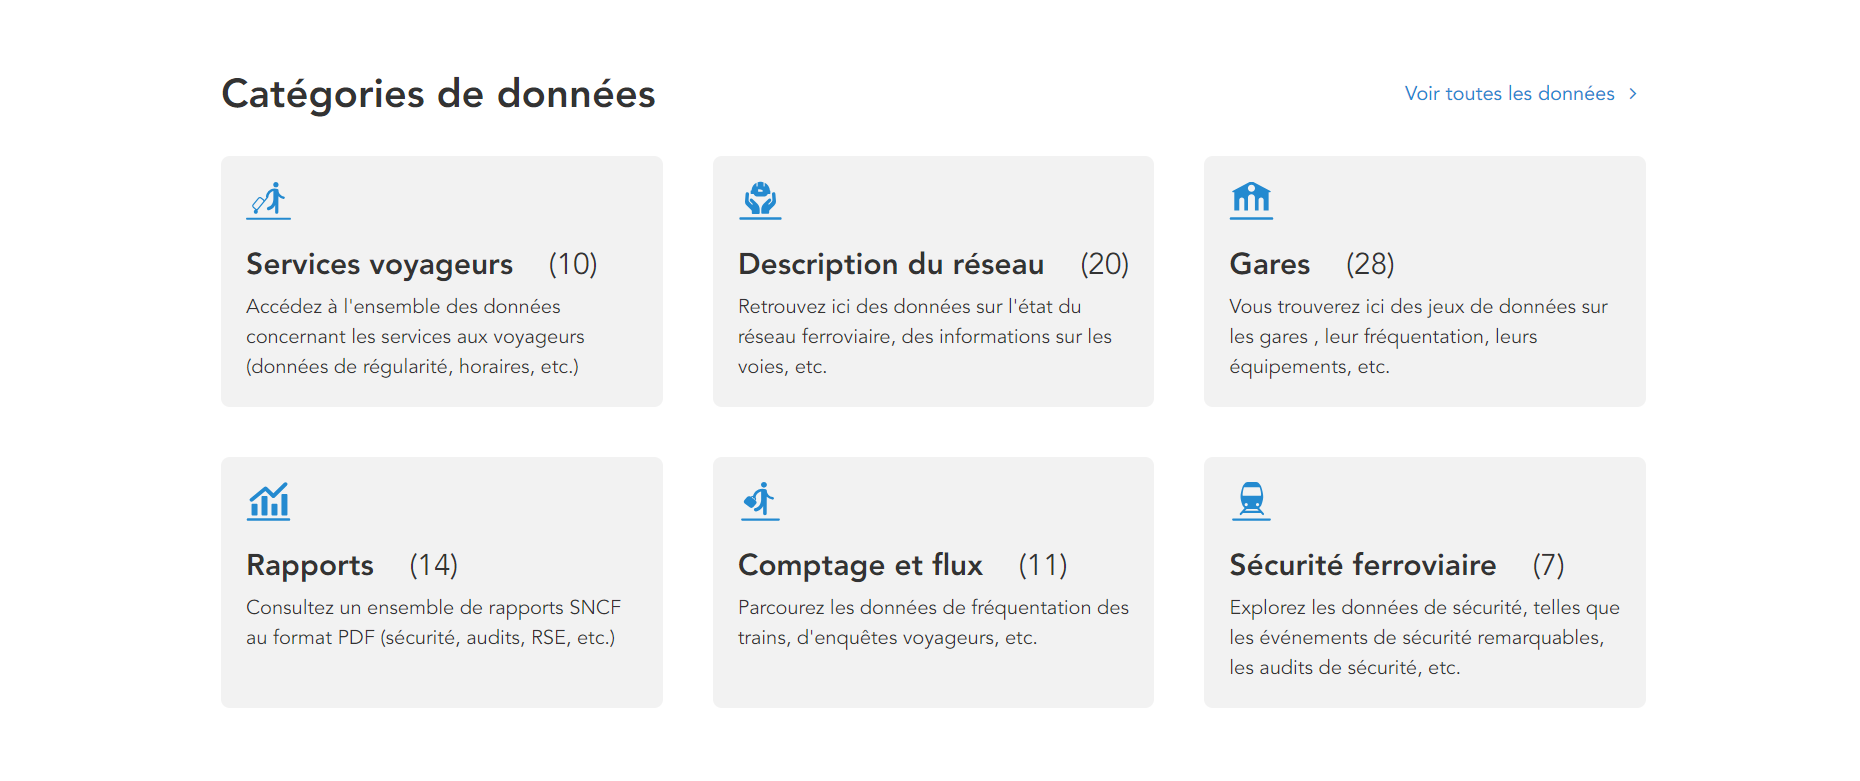
\includegraphics{images/categories-donnees.png}

Ces données concernent des objets possedés par la SNCF (gares, objets)
mais aussi des enquêtes réalisées sur des individus anonymement
(fréquentation, voyageurs). Les données sont liées à une période
temporelle précise de \textbf{2017 à 2022}.

\begin{quote}
L'ensemble des données brutes sont accessibles depuis le dossier /data.
\end{quote}

\textbf{Nombre d'observations}

Le nombre d'observations varie selon chaque jeu de données. Pour plus de
détail, nous avons détaillé précisement le nombre d'observations dont
nous disposions.

\begin{longtable}[]{@{}
  >{\raggedright\arraybackslash}p{(\columnwidth - 8\tabcolsep) * \real{0.1944}}
  >{\raggedright\arraybackslash}p{(\columnwidth - 8\tabcolsep) * \real{0.1944}}
  >{\raggedright\arraybackslash}p{(\columnwidth - 8\tabcolsep) * \real{0.1944}}
  >{\raggedright\arraybackslash}p{(\columnwidth - 8\tabcolsep) * \real{0.2222}}
  >{\raggedright\arraybackslash}p{(\columnwidth - 8\tabcolsep) * \real{0.1944}}@{}}
\toprule\noalign{}
\begin{minipage}[b]{\linewidth}\raggedright
---
\end{minipage} & \begin{minipage}[b]{\linewidth}\raggedright
Nom du dataset
\end{minipage} & \begin{minipage}[b]{\linewidth}\raggedright
Nombre d'observations
\end{minipage} & \begin{minipage}[b]{\linewidth}\raggedright
Lien
\end{minipage} & \begin{minipage}[b]{\linewidth}\raggedright
Description
\end{minipage} \\
\midrule\noalign{}
\endhead
\bottomrule\noalign{}
\endlastfoot
01 & dataset1-gares-de-voyageurs.csv & 2.862 &
\href{https://data.sncf.com/explore/dataset/gares-de-voyageurs/export/}{Dataset1}
& Jeu de données sur les gares de voyageurs \\
02 & dataset2-frequentation-gares.csv & 21.147 &
\href{https://data.sncf.com/explore/dataset/frequentation-gares/export/}{Dataset2}
& Jeu de données sur la fréquentation des gares \\
03 & dataset3-motif-deplacement.csv & 284 &
\href{https://data.sncf.com/explore/dataset/motif-deplacement/export/}{Dataset3}
& Jeu de données sur les motifs de déplacement \\
04 &
dataset4-enquetes-gares-connexions-repartition-par-repartition-par-categories-socio-profe.csv
& 697 &
\href{https://data.sncf.com/explore/dataset/enquetes-gares-connexions-repartition-par-repartition-par-categories-socio-profe/export/}{Dataset4}
& Jeu de données sur les CSP des voyageurs \\
05 &
dataset5-enquetes-gares-connexions-repartition-repartition-par-classe-dage.csv
& 375 &
\href{https://data.sncf.com/explore/dataset/enquetes-gares-connexions-repartition-repartition-par-classe-dage/export/}{Dataset5}
& Jeu de données sur l'âge des voyageurs \\
06 & dataset6-objets-trouves-gares.csv & 1.844.912 &
\href{https://data.sncf.com/explore/dataset/objets-trouves-gares/export/}{Dataset6}
& Jeu de données sur les objets trouvés en gare \\
07 & dataset7-objets-trouves-restitution.csv & 858.180 &
\href{https://data.sncf.com/explore/dataset/objets-trouves-restitution/export/}{Dataset7}
& Jeu de données sur les objets restitués \\
\end{longtable}

Au sein de ces données nous constatons que toutes s'orchestrent autour
d'une donnée principale (Gare, 01) qui est présent dans tous les
datasets. Nous pouvons donc segmenter les données restantes par des
critères géographiques (02,03,04,05), des critères temporels (06,07),
des critères voyageurs (08,09,10,11,12,13,14) et des critères sur les
objets perdus/trouvés (15,16,17).

\textbf{Variables}

Nous avons décidé d'utiliser \textbf{17 variables} pour notre projet
provenant des jeux de données bruts ou alors d'attributs crées par nos
soins.

\begin{longtable}[]{@{}
  >{\raggedright\arraybackslash}p{(\columnwidth - 10\tabcolsep) * \real{0.1549}}
  >{\raggedright\arraybackslash}p{(\columnwidth - 10\tabcolsep) * \real{0.1549}}
  >{\raggedright\arraybackslash}p{(\columnwidth - 10\tabcolsep) * \real{0.1549}}
  >{\raggedright\arraybackslash}p{(\columnwidth - 10\tabcolsep) * \real{0.1549}}
  >{\raggedright\arraybackslash}p{(\columnwidth - 10\tabcolsep) * \real{0.1549}}
  >{\raggedright\arraybackslash}p{(\columnwidth - 10\tabcolsep) * \real{0.2254}}@{}}
\toprule\noalign{}
\begin{minipage}[b]{\linewidth}\raggedright
---
\end{minipage} & \begin{minipage}[b]{\linewidth}\raggedright
Nom de la variable
\end{minipage} & \begin{minipage}[b]{\linewidth}\raggedright
Type
\end{minipage} & \begin{minipage}[b]{\linewidth}\raggedright
Format
\end{minipage} & \begin{minipage}[b]{\linewidth}\raggedright
Dataset (Origine)
\end{minipage} & \begin{minipage}[b]{\linewidth}\raggedright
Description
\end{minipage} \\
\midrule\noalign{}
\endhead
\bottomrule\noalign{}
\endlastfoot
01 & gare & Nominale & String & 1,2,3,4,5,6,7 & Nom de la gare \\
02 & departement & Ordinale & NN & 1 & Numéro du département \\
03 & zone & Nominale & \{A,B,C\} & 1 & Lettre correspondant à la zone
géographique \\
04 & latitude & Continue & M''S'NS & 1 & Latitude de l'objet gare \\
05 & longitude & Continue & M''S'NS & 1 & Longitude de l'objet gare \\
06 & annee & Ordinale & YYYY & 2,3,4 & Année correspondante \\
07 & timing\_reception & Discrète & YYYY-MM-DD-HH-MM-SS & 6,7 &
Réception de l'objet perdu \\
08 & nb\_voyageurs & Discrète & Integer & 2 & Nombre de voyageurs \\
09 & age & Ordinale & String & 5 & Age d'un voyageur \\
10 & pourcentage\_age & Continue & \% & 5 & Pourcentage sur l'âge des
voyageurs \\
11 & csp & Nominale & String & 4 & Catégorie socio-professionnel d'un
voyageur \\
12 & pourcentage\_csp & Continue & \% & 4 & Pourcentage sur la catégorie
socio-professionnel des voyageurs \\
13 & motif\_deplacement & Nominale & String & 3 & Motif de déplacement
d'un voyageur \\
14 & pourcentage\_deplacement & Continue & \% & 3 & Pourcentage sur le
motif de déplacement des voyageurs \\
15 & nature\_objet & Nominale & String & 6,7 & Nature de l'objet \\
16 & categorie\_objet & Nominale & String & 6,7 & Catégorie de
l'objet \\
17 & code\_uic & Nominale & NNNNNNNNNN & 6,7 & Code UIC de la gare \\
\end{longtable}

\textbf{Variables particulières}

Notre jeu de données comprenant des coordonnées spatiales, nous avons
estimé qu'il était intéressant de réaliser des cartes. En effet, les
coordonnées géographiques de longitude et latitude pourront être
utilisée pour catographier le réseau des gares françaises.

L'ensemble des données énoncées plus en haut nous paraissent pertinentes
dans le cadre d'une étude. En effet, elles permettent :

\begin{itemize}
\tightlist
\item
  d'étudier les effets de la fréquentation sur les vols/pertes d'objets
\item
  d'effectuer une analyse temporelle et spatiale du réseau
\item
  d'effectuer des classements et des comparaisons entre les différentes
  régions et/ou départements (analyse multiscalaire). Exemple : espace
  moins déservi par exemple.
\end{itemize}

\hypertarget{plan-danalyse}{%
\subsection{Plan d'analyse}\label{plan-danalyse}}

\begin{enumerate}
\def\labelenumi{\arabic{enumi}.}
\item
  \textbf{Découverte du jeu de données} et surtout comprendre à quoi
  servent nos données. Par exemple : nous souhaitons réaliser des
  visualisations sur le réseau ferroviaire actuel, étudier la
  répartition générale des voyageurs\ldots{} \textgreater{} A quoi
  ressemble le réseau SNCF en France ? Quels sont les départements les
  mieux équipés ? A quel point Paris a une place importante dans le
  réseau des autres territoires ?
\item
  \textbf{Analyse des voyageurs} : De façon plus précise, nous
  étudierons les voyageurs qui utilisent quotidiennement les réseaux
  ferrés français. Cela passera notamment par des attributs d'âge, de
  CSP ou encore de motif de déplacement. \textgreater{} Le nombre de
  voyageurs est-il bien repartis entre les gares d'un même département ?
  Quel est le voyageur moyen de la SNCF ? Comment ce voyageur diffère en
  fonction des gares ? Quel est la relation entre les motifs de voyage
  des passagers et leur répartition par âge et par profession ?
\item
  \textbf{Analyse des objets} : De la même façon, nous souhaiterions
  étudier les objets perdus en gares. Pour cela, nous utiliserons
  également un second jeu de données sur les objets retrouvés.
  \textgreater{} Y-a-t-il plus de chances de perdre un objet selon la
  gare ? Doit-on s'attendre à un afflux d'objets perdus plus important
  dans les mois de Juillet-Août 2024 plus important que les dernières
  années ? Quelles sont les chances de retrouver un objet perdu ?
  Quelles sont les chances de retrouver un objet en fonction de sa
  nature ?
\item
  \textbf{Analyse spatiale} : A l'aide de nos données spatiales, nous
  souhaitons réaliser des cartes. Ces dernières permettront visuellement
  de voir la disposition et la répartition des gares en France
  Métropolitaine.
\item
  Enfin si nous souhaitons \textbf{rajouter des questions}, nous nous
  laissons la liberté de les rajouter au plan d'analyse.
\end{enumerate}

\begin{Shaded}
\begin{Highlighting}[]
\FunctionTok{library}\NormalTok{(ggplot2)}
\FunctionTok{library}\NormalTok{(dplyr)}
\end{Highlighting}
\end{Shaded}

\begin{verbatim}
## 
## Attachement du package : 'dplyr'
\end{verbatim}

\begin{verbatim}
## Les objets suivants sont masqués depuis 'package:stats':
## 
##     filter, lag
\end{verbatim}

\begin{verbatim}
## Les objets suivants sont masqués depuis 'package:base':
## 
##     intersect, setdiff, setequal, union
\end{verbatim}

\begin{Shaded}
\begin{Highlighting}[]
\FunctionTok{library}\NormalTok{(tidyr)}
\FunctionTok{library}\NormalTok{(tibble)}
\FunctionTok{library}\NormalTok{(readr)}
\FunctionTok{library}\NormalTok{(lubridate)}
\end{Highlighting}
\end{Shaded}

\begin{verbatim}
## 
## Attachement du package : 'lubridate'
\end{verbatim}

\begin{verbatim}
## Les objets suivants sont masqués depuis 'package:base':
## 
##     date, intersect, setdiff, union
\end{verbatim}

\begin{Shaded}
\begin{Highlighting}[]
\FunctionTok{library}\NormalTok{(forcats)}
\FunctionTok{library}\NormalTok{(stringr)}
\FunctionTok{library}\NormalTok{(sf)}
\end{Highlighting}
\end{Shaded}

\begin{verbatim}
## Linking to GEOS 3.11.2, GDAL 3.8.2, PROJ 9.3.1; sf_use_s2() is TRUE
\end{verbatim}

\begin{Shaded}
\begin{Highlighting}[]
\FunctionTok{library}\NormalTok{(rnaturalearth)}
\FunctionTok{library}\NormalTok{(rnaturalearthdata)}
\end{Highlighting}
\end{Shaded}

\begin{verbatim}
## 
## Attachement du package : 'rnaturalearthdata'
\end{verbatim}

\begin{verbatim}
## L'objet suivant est masqué depuis 'package:rnaturalearth':
## 
##     countries110
\end{verbatim}

\hypertarget{nettoyage-des-donnuxe9es}{%
\section{Nettoyage des données}\label{nettoyage-des-donnuxe9es}}

Le \textbf{nettoyage des données} est la première étapes de notre
projet. C'est ici que nous allons créer de nouvelles tables, modifier
les jeux de données existants (supprimer ou renommer les colonnes
existantes). \emph{{[}TODO{]} Ajouter des explications sur la complexité
de nos données}

Afin de travailler proprement, nous avons réaliser les étapes suivantes
:

\begin{enumerate}
\def\labelenumi{\arabic{enumi}.}
\item
  Nous avons commencé par \textbf{observer les colonnes} de nos jeux de
  données. Nous avons pu isoler lesquels étaient susceptibles d'être
  utilisées. Nous les avons ensuite \textbf{importées}.
\item
  Ensuite, nous avons choisi de \textbf{renommer les colonnes} de nos
  jeux de données selon une norme précise (voir \textbf{Convention de
  nommage des colonnes} ci-dessous). Les colonnes de base des tables
  utilisaient des espaces, ce qui est incompatible avec l'appel de ces
  dernières.
\item
  Une fois les tables modifiées, nous avons du \textbf{filtrer nos
  données}.
\end{enumerate}

\textbf{Convention de nommage des colonnes} - Transformer les espaces en
underscore. - Nommer les variables avec des minuscules.

\begin{quote}
Exemple : Code Postal en code\_postal
\end{quote}

\emph{{[}TODO{]} Rajouter des données les tables modifiées ici}

\hypertarget{importation-des-jeux-de-donnuxe9es}{%
\subsection{Importation des jeux de
données}\label{importation-des-jeux-de-donnuxe9es}}

\begin{Shaded}
\begin{Highlighting}[]
\NormalTok{gares }\OtherTok{\textless{}{-}} \FunctionTok{read\_delim}\NormalTok{(}\AttributeTok{file =} \StringTok{"data/dataset1{-}gares{-}de{-}voyageurs.csv"}\NormalTok{, }\AttributeTok{delim=}\StringTok{";"}\NormalTok{)}
\end{Highlighting}
\end{Shaded}

\begin{verbatim}
## Rows: 2862 Columns: 5
## -- Column specification --------------------------------------------------------
## Delimiter: ";"
## chr (4): Nom, Trigramme, Segment DRG, Position géographique
## dbl (1): Code commune
## 
## i Use `spec()` to retrieve the full column specification for this data.
## i Specify the column types or set `show_col_types = FALSE` to quiet this message.
\end{verbatim}

\begin{Shaded}
\begin{Highlighting}[]
\NormalTok{frequentation }\OtherTok{\textless{}{-}} \FunctionTok{read\_delim}\NormalTok{(}\AttributeTok{file =} \StringTok{"data/dataset2{-}frequentation{-}gares.csv"}\NormalTok{, }\AttributeTok{delim=}\StringTok{";"}\NormalTok{)}
\end{Highlighting}
\end{Shaded}

\begin{verbatim}
## Rows: 3021 Columns: 20
## -- Column specification --------------------------------------------------------
## Delimiter: ";"
## chr  (2): Nom de la gare, Segmentation DRG
## dbl (18): Code UIC, Code postal, Total Voyageurs 2022, Total Voyageurs + Non...
## 
## i Use `spec()` to retrieve the full column specification for this data.
## i Specify the column types or set `show_col_types = FALSE` to quiet this message.
\end{verbatim}

\begin{Shaded}
\begin{Highlighting}[]
\NormalTok{motif\_depl }\OtherTok{\textless{}{-}} \FunctionTok{read\_delim}\NormalTok{(}\AttributeTok{file =} \StringTok{"data/dataset3{-}motif{-}deplacement.csv"}\NormalTok{, }\AttributeTok{delim=}\StringTok{";"}\NormalTok{)}
\end{Highlighting}
\end{Shaded}

\begin{verbatim}
## Rows: 284 Columns: 5
## -- Column specification --------------------------------------------------------
## Delimiter: ";"
## chr (2): Gare enquêtée, Motif du déplacement
## dbl (3): UIC, POURCENTAGE, Année
## 
## i Use `spec()` to retrieve the full column specification for this data.
## i Specify the column types or set `show_col_types = FALSE` to quiet this message.
\end{verbatim}

\begin{Shaded}
\begin{Highlighting}[]
\NormalTok{CSP\_voya }\OtherTok{\textless{}{-}} \FunctionTok{read\_delim}\NormalTok{(}\AttributeTok{file =} \StringTok{"data/dataset4{-}enquetes{-}gares{-}connexions{-}repartition{-}par{-}repartition{-}par{-}categories{-}socio{-}profe.csv"}\NormalTok{, }\AttributeTok{delim=}\StringTok{";"}\NormalTok{)}
\end{Highlighting}
\end{Shaded}

\begin{verbatim}
## Rows: 697 Columns: 5
## -- Column specification --------------------------------------------------------
## Delimiter: ";"
## chr (2): Gare enquêtée, CSP
## dbl (3): UIC, Pourcentage, Année
## 
## i Use `spec()` to retrieve the full column specification for this data.
## i Specify the column types or set `show_col_types = FALSE` to quiet this message.
\end{verbatim}

\begin{Shaded}
\begin{Highlighting}[]
\NormalTok{age\_voya }\OtherTok{\textless{}{-}} \FunctionTok{read\_delim}\NormalTok{(}\AttributeTok{file =} \StringTok{"data/dataset5{-}enquetes{-}gares{-}connexions{-}repartition{-}repartition{-}par{-}classe{-}dage.csv"}\NormalTok{, }\AttributeTok{delim=}\StringTok{";"}\NormalTok{)}
\end{Highlighting}
\end{Shaded}

\begin{verbatim}
## Rows: 375 Columns: 5
## -- Column specification --------------------------------------------------------
## Delimiter: ";"
## chr (2): Gare enquêtée, Classe d'âge
## dbl (3): UIC, Pourcentage, Année
## 
## i Use `spec()` to retrieve the full column specification for this data.
## i Specify the column types or set `show_col_types = FALSE` to quiet this message.
\end{verbatim}

\begin{Shaded}
\begin{Highlighting}[]
\NormalTok{obj\_perdus }\OtherTok{\textless{}{-}} \FunctionTok{read\_delim}\NormalTok{(}\AttributeTok{file =} \StringTok{"data/dataset6{-}objets{-}trouves{-}gares.csv"}\NormalTok{, }\AttributeTok{delim=}\StringTok{";"}\NormalTok{)}
\end{Highlighting}
\end{Shaded}

\begin{verbatim}
## Rows: 1876131 Columns: 6
## -- Column specification --------------------------------------------------------
## Delimiter: ";"
## chr  (5): Gare, Code UIC, Nature d'objets, Type d'objets, Type d'enregistrement
## dttm (1): Date de la déclaration de perte
## 
## i Use `spec()` to retrieve the full column specification for this data.
## i Specify the column types or set `show_col_types = FALSE` to quiet this message.
\end{verbatim}

\begin{Shaded}
\begin{Highlighting}[]
\NormalTok{obj\_trouves }\OtherTok{\textless{}{-}} \FunctionTok{read\_delim}\NormalTok{(}\AttributeTok{file =} \StringTok{"data/dataset7{-}objets{-}trouves{-}restitution.csv"}\NormalTok{, }\AttributeTok{delim=}\StringTok{";"}\NormalTok{)}
\end{Highlighting}
\end{Shaded}

\begin{verbatim}
## Rows: 867912 Columns: 7
## -- Column specification --------------------------------------------------------
## Delimiter: ";"
## chr  (5): Gare, Code UIC, Nature d'objets, Type d'objets, Type d'enregistrement
## dttm (2): Date, Date et heure de restitution
## 
## i Use `spec()` to retrieve the full column specification for this data.
## i Specify the column types or set `show_col_types = FALSE` to quiet this message.
\end{verbatim}

\begin{Shaded}
\begin{Highlighting}[]
\CommentTok{\#Nettoyage des données pour le traitement}
\NormalTok{gares\_clean }\OtherTok{\textless{}{-}}\NormalTok{ gares }\SpecialCharTok{\%\textgreater{}\%}
  \FunctionTok{separate}\NormalTok{(}\StringTok{"Position géographique"}\NormalTok{, }\AttributeTok{into =} \FunctionTok{c}\NormalTok{(}\StringTok{"Latitude"}\NormalTok{, }\StringTok{"Longitude"}\NormalTok{), }\AttributeTok{sep =} \StringTok{", "}\NormalTok{) }\SpecialCharTok{\%\textgreater{}\%}
  \FunctionTok{mutate}\NormalTok{(}\FunctionTok{across}\NormalTok{(}\FunctionTok{c}\NormalTok{(Latitude, Longitude), as.numeric)) }\SpecialCharTok{\%\textgreater{}\%}
  \FunctionTok{rename}\NormalTok{(}\AttributeTok{Gare =} \StringTok{"Nom"}\NormalTok{, }\AttributeTok{Code\_Postal =} \StringTok{"Code commune"}\NormalTok{, }\AttributeTok{Zones\_vac =} \StringTok{"Segment DRG"}\NormalTok{)}

\NormalTok{frequentation\_clean }\OtherTok{\textless{}{-}}\NormalTok{ frequentation }\SpecialCharTok{\%\textgreater{}\%}
  \FunctionTok{rename\_with}\NormalTok{(}\AttributeTok{.cols =} \FunctionTok{contains}\NormalTok{(}\StringTok{"Non"}\NormalTok{), }
              \SpecialCharTok{\textasciitilde{}} \FunctionTok{sub}\NormalTok{(}\StringTok{\textquotesingle{}Total Voyageurs }\SpecialCharTok{\textbackslash{}\textbackslash{}}\StringTok{+ Non voyageurs\textquotesingle{}}\NormalTok{, }\StringTok{"Personnes"}\NormalTok{, .))}\SpecialCharTok{\%\textgreater{}\%}
  \FunctionTok{rename\_with}\NormalTok{(}\AttributeTok{.cols =} \FunctionTok{contains}\NormalTok{(}\StringTok{"Total"}\NormalTok{), }
              \SpecialCharTok{\textasciitilde{}} \FunctionTok{sub}\NormalTok{(}\StringTok{\textquotesingle{}Total Voyageurs\textquotesingle{}}\NormalTok{, }\StringTok{"Voyageurs"}\NormalTok{, .))}\SpecialCharTok{\%\textgreater{}\%}
  \FunctionTok{pivot\_longer}\NormalTok{(}\AttributeTok{cols =} \FunctionTok{starts\_with}\NormalTok{(}\StringTok{"Personnes"}\NormalTok{) }\SpecialCharTok{|} \FunctionTok{starts\_with}\NormalTok{(}\StringTok{"Voyageurs"}\NormalTok{), }
               \AttributeTok{names\_to =} \FunctionTok{c}\NormalTok{(}\StringTok{".value"}\NormalTok{, }\StringTok{"Année"}\NormalTok{), }
               \AttributeTok{names\_sep =} \StringTok{" "}\NormalTok{)}\SpecialCharTok{\%\textgreater{}\%}
  \FunctionTok{mutate}\NormalTok{(Année }\OtherTok{=} \FunctionTok{as.numeric}\NormalTok{(Année))}\SpecialCharTok{\%\textgreater{}\%}
  \FunctionTok{rename}\NormalTok{(}\AttributeTok{Gare =} \StringTok{"Nom de la gare"}\NormalTok{, }\AttributeTok{UIC =} \StringTok{"Code UIC"}\NormalTok{, }\AttributeTok{Code\_Postal =} \StringTok{"Code postal"}\NormalTok{, }\AttributeTok{Zones\_vac =} \StringTok{"Segmentation DRG"}\NormalTok{)}\SpecialCharTok{\%\textgreater{}\%}
  \FunctionTok{mutate}\NormalTok{(}\AttributeTok{UIC =} \FunctionTok{as.character}\NormalTok{(UIC)) }\SpecialCharTok{\%\textgreater{}\%}
  \FunctionTok{mutate}\NormalTok{(}\AttributeTok{UIC =} \FunctionTok{substr}\NormalTok{(UIC, }\DecValTok{3}\NormalTok{, }\DecValTok{8}\NormalTok{)) }\SpecialCharTok{\%\textgreater{}\%}
  \FunctionTok{mutate}\NormalTok{(Département }\OtherTok{=} \FunctionTok{substr}\NormalTok{(Code\_Postal, }\DecValTok{1}\NormalTok{, }\DecValTok{2}\NormalTok{))}
  
\FunctionTok{View}\NormalTok{(frequentation\_clean)}

\NormalTok{age\_voya\_clean }\OtherTok{\textless{}{-}}\NormalTok{ age\_voya }\SpecialCharTok{\%\textgreater{}\%}
  \FunctionTok{rename}\NormalTok{(}\AttributeTok{Gare =} \StringTok{\textasciigrave{}}\AttributeTok{Gare enquêtée}\StringTok{\textasciigrave{}}\NormalTok{)}\SpecialCharTok{\%\textgreater{}\%}
  \FunctionTok{mutate}\NormalTok{(}\AttributeTok{UIC =} \FunctionTok{as.character}\NormalTok{(UIC))}
  

\NormalTok{gares\_freq\_clean }\OtherTok{\textless{}{-}}\NormalTok{ gares\_clean }\SpecialCharTok{\%\textgreater{}\%} 
  \FunctionTok{inner\_join}\NormalTok{(frequentation\_clean, }\AttributeTok{by =} \StringTok{"Gare"}\NormalTok{)}
\CommentTok{\#Création du template de la France}
\NormalTok{france }\OtherTok{\textless{}{-}} \FunctionTok{ne\_countries}\NormalTok{(}\AttributeTok{scale=}\StringTok{"medium"}\NormalTok{, }\AttributeTok{country =} \StringTok{"France"}\NormalTok{, }\AttributeTok{returnclass=}\StringTok{"sf"}\NormalTok{)}\SpecialCharTok{\%\textgreater{}\%}
  \FunctionTok{st\_crop}\NormalTok{(}\AttributeTok{xmin =} \SpecialCharTok{{-}}\FloatTok{5.2}\NormalTok{, }\AttributeTok{xmax =} \FloatTok{9.7}\NormalTok{, }\AttributeTok{ymin =} \DecValTok{41}\NormalTok{, }\AttributeTok{ymax =} \DecValTok{51}\NormalTok{)  }\CommentTok{\# Limites de la France métropolitaine}
\end{Highlighting}
\end{Shaded}

\begin{verbatim}
## Warning: attribute variables are assumed to be spatially constant throughout
## all geometries
\end{verbatim}

\hypertarget{duxe9couverte}{%
\section{Découverte}\label{duxe9couverte}}

Dans cette partie, nous découvrirons le jeu de données.

\textbf{Visualisations réalisées}

\begin{enumerate}
\def\labelenumi{\arabic{enumi}.}
\item
  Fréquentation des gares
\item
  Carte de la fréquentation des gares en France Métropolitaine
\end{enumerate}

{[}TODO{]} à compléter

\begin{quote}
L'ensemble des visualisations sont réalisées avec les données de l'année
\textbf{2022}, car ce sont les données les plus récentes à notre
disposition.
\end{quote}

\emph{À quoi ressemble le réseau SNCF en France ? Quels sont les
départements les mieux équipés ? À quel point Paris a une place
importante dans le réseau des autres territoires ?}

\hypertarget{fruxe9quentation-des-gares}{%
\subsection{1. Fréquentation des
gares}\label{fruxe9quentation-des-gares}}

Tout d'abord, voici un petit tour d'horizon du dataset
\textbf{Frequentation}.

\begin{Shaded}
\begin{Highlighting}[]
\FunctionTok{head}\NormalTok{(frequentation\_clean)}
\end{Highlighting}
\end{Shaded}

\begin{verbatim}
## # A tibble: 6 x 8
##   Gare     UIC    Code_Postal Zones_vac Année Personnes Voyageurs Département
##   <chr>    <chr>        <dbl> <chr>     <dbl>     <dbl>     <dbl> <chr>      
## 1 Abbaretz 481614       44170 C          2022     40825     40825 44         
## 2 Abbaretz 481614       44170 C          2021     27466     27466 44         
## 3 Abbaretz 481614       44170 C          2020     22773     22773 44         
## 4 Abbaretz 481614       44170 C          2019     38473     38473 44         
## 5 Abbaretz 481614       44170 C          2018     38027     38027 44         
## 6 Abbaretz 481614       44170 C          2017     35637     35637 44
\end{verbatim}

\begin{Shaded}
\begin{Highlighting}[]
\FunctionTok{summary}\NormalTok{(frequentation\_clean)}
\end{Highlighting}
\end{Shaded}

\begin{verbatim}
##      Gare               UIC             Code_Postal     Zones_vac        
##  Length:24168       Length:24168       Min.   : 1000   Length:24168      
##  Class :character   Class :character   1st Qu.:31770   Class :character  
##  Mode  :character   Mode  :character   Median :58320   Mode  :character  
##                                        Mean   :53024                     
##                                        3rd Qu.:74310                     
##                                        Max.   :98000                     
##      Année        Personnes           Voyageurs         Département       
##  Min.   :2015   Min.   :        0   Min.   :        0   Length:24168      
##  1st Qu.:2017   1st Qu.:     7335   1st Qu.:     7335   Class :character  
##  Median :2018   Median :    41005   Median :    40909   Mode  :character  
##  Mean   :2018   Mean   :   898228   Mean   :   807825                     
##  3rd Qu.:2020   3rd Qu.:   260290   3rd Qu.:   218036                     
##  Max.   :2022   Max.   :278140181   Max.   :247963153
\end{verbatim}

Nous avons choisi d'utiliser des données discrètes (nombre de voyageurs)
en abscisse et nominales (gares) en ordonnée. Afin de constater les
différences entre les gares, une comparaison basée sur un bar chart a
été réalisée ci-dessous.

De plus, afin d'obtenir un classement des gares les plus fréquentées,
nous avons choisi de filtrer le dataset pour ne garder que les gares au
dessus d'un seuil de 20.000.000 individus. Ce filtre nous permet de
faire ressortir les gares les plus fréquentées uniquement.

\begin{Shaded}
\begin{Highlighting}[]
\NormalTok{freq }\OtherTok{\textless{}{-}}\NormalTok{ frequentation\_clean }\SpecialCharTok{\%\textgreater{}\%}
  \FunctionTok{select}\NormalTok{(Gare, Voyageurs, Année) }\SpecialCharTok{\%\textgreater{}\%}
  \FunctionTok{filter}\NormalTok{(Voyageurs }\SpecialCharTok{\textgreater{}} \DecValTok{20000000}\NormalTok{) }\SpecialCharTok{\%\textgreater{}\%}
  \FunctionTok{filter}\NormalTok{(Année }\SpecialCharTok{==} \StringTok{"2022"}\NormalTok{)}

\FunctionTok{ggplot}\NormalTok{(}\AttributeTok{data =}\NormalTok{ freq, }\AttributeTok{mapping =} \FunctionTok{aes}\NormalTok{(}\AttributeTok{x=}\NormalTok{Voyageurs,}\AttributeTok{y=}\NormalTok{Gare)) }\SpecialCharTok{+}
  \FunctionTok{geom\_col}\NormalTok{() }\SpecialCharTok{+}
  \FunctionTok{theme\_minimal}\NormalTok{() }\SpecialCharTok{+}
  \FunctionTok{labs}\NormalTok{(}\AttributeTok{title =} \StringTok{"Fréquentation par gare (2022)"}\NormalTok{,}
       \AttributeTok{subtitle =} \StringTok{"\textless{} minimum 20.000.000 de voyageurs \textgreater{}"}\NormalTok{,}
       \AttributeTok{x =} \StringTok{"Nombre de voyageurs"}\NormalTok{,}
       \AttributeTok{y =} \StringTok{"Gares"}\NormalTok{)}
\end{Highlighting}
\end{Shaded}

\includegraphics{rogue-one_files/figure-latex/unnamed-chunk-4-1.pdf}

\textbf{Analyse} On remarque que les gares avec le plus de fréquentation
sont les gares parisiennes. En termes de positionnement, nous retrouvons
: Gare du Nord (1), Gare Saint-Lazare (2), Gare de Lyon (3), Gare
Montparnasse (4). D'autres gares se démarquent mais restent sensiblement
proches les unes des autres.

Cette visualisation n'est pas étonnante si l'on utilise régulièrement le
réseau RATP et SNCF en Ile de France. En effet, la grande majorité des
trajets partent de Paris et arrivent sur Paris.

Gare du Nord semble être la gare la plus fréquentée du réseau. En
faisant des recherches, on apprend qu'elle permet des départs vers le
Royaume-Uni (Londres-St-Pancras), la Belgique (Bruxelles-Midi) ou encore
les Pays-Bas (Amsterdam-Centraal) \emph{(Figure 1)}. La population est
généralement importante dans ces grandes villes et capitales
européennes, ce qui explique également la fréquentation de Gare du Nord
que ce soit pour des trajets professionnels ou touristiques.

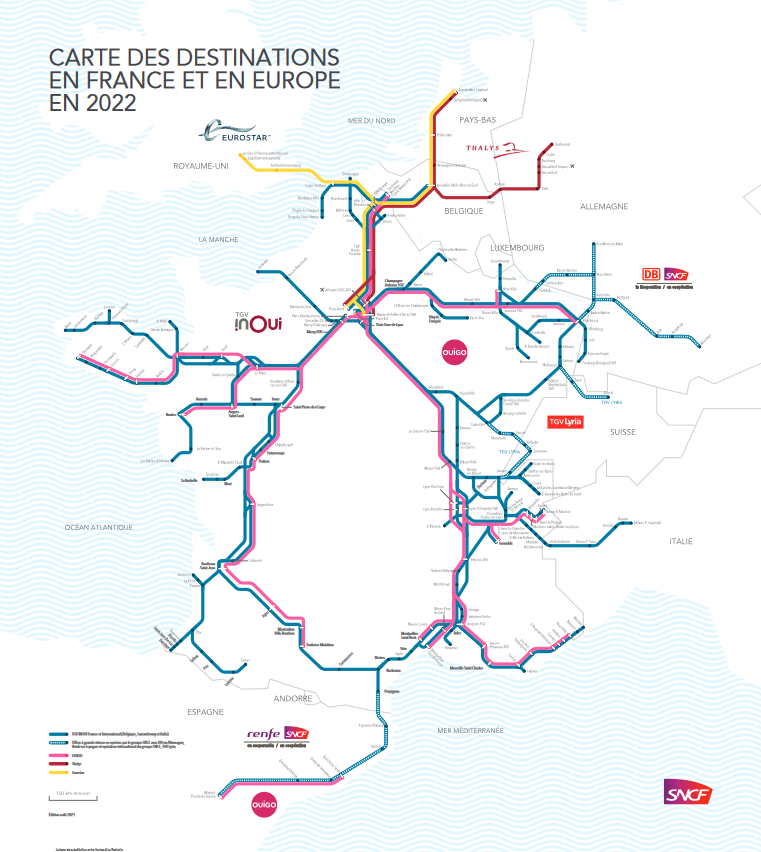
\includegraphics[width=5.20833in,height=\textheight]{images/carte-reseau-sncf.png}

Figure 1. Carte des destinations en France et en Europe (2022)

Source :
\url{https://www.sncf-connect.com/aide/le-reseau-sncf-en-france-et-en-europe}

\hypertarget{carte-de-la-fruxe9quentation-des-gares-en-france-muxe9tropolitaine}{%
\subsection{2. Carte de la fréquentation des gares en France
Métropolitaine}\label{carte-de-la-fruxe9quentation-des-gares-en-france-muxe9tropolitaine}}

{[}TODO{]} est ce qu'on laisse la couleur ? pertinent de décrire par
année en couleur alors qu'on dit que c'est en 2022

Pour poursuivre notre découverte du réseau SNCF, nous avons choisi de
représenter la fréquentation des gares sur une carte de France
Métropolitaine. Avec cette visualisation cartographique, on peut
comprendre plus spatialement les enjeux liés aux flux de voyageurs en
2022.

Pour représenter cela, on utilise des données discrètes (longitude,
latitude, nombre de voyageurs) et ordinales (année) sur une carte. Etant
donné qu'il s'agit d'une carte, on place la longitude en abscisse et la
latitude en ordonnée. De plus, on a ajouté de la couleur afin de faire
ressortir des gares qui n'ont plus vraiment de fréquentation en 2022.

\begin{Shaded}
\begin{Highlighting}[]
\FunctionTok{ggplot}\NormalTok{(}\AttributeTok{data =}\NormalTok{ france) }\SpecialCharTok{+}
  \FunctionTok{geom\_sf}\NormalTok{(}\AttributeTok{fill =} \StringTok{"white"}\NormalTok{, }\AttributeTok{color =} \StringTok{"black"}\NormalTok{) }\SpecialCharTok{+}
  \FunctionTok{geom\_point}\NormalTok{(}\AttributeTok{data =}\NormalTok{ gares\_freq\_clean, }\FunctionTok{aes}\NormalTok{(}\AttributeTok{x =}\NormalTok{ Longitude, }\AttributeTok{y =}\NormalTok{ Latitude, }\AttributeTok{size=}\NormalTok{Voyageurs, }\AttributeTok{color =}\NormalTok{ Année), }\AttributeTok{alpha =} \FloatTok{0.7}\NormalTok{) }\SpecialCharTok{+}
  \FunctionTok{scale\_size\_continuous}\NormalTok{(}
    \AttributeTok{range =} \FunctionTok{c}\NormalTok{(}\DecValTok{1}\NormalTok{,}\DecValTok{8}\NormalTok{), }
\NormalTok{  ) }\SpecialCharTok{+}
  \FunctionTok{theme\_minimal}\NormalTok{() }\SpecialCharTok{+}
  \FunctionTok{labs}\NormalTok{(}\AttributeTok{title =} \StringTok{"Fréquentation par gare (2022)"}\NormalTok{,}
       \AttributeTok{x =} \StringTok{"Longitude"}\NormalTok{,}
       \AttributeTok{y =} \StringTok{"Latitude"}\NormalTok{,}
       \AttributeTok{size =} \StringTok{"Fréquentation"}\NormalTok{)}
\end{Highlighting}
\end{Shaded}

\includegraphics{rogue-one_files/figure-latex/unnamed-chunk-5-1.pdf}

\textbf{Analyse} Au premier abord, on remarque que les gares tracent
d'elles même, sur la carte, la majeur partie du réseau ferroviaire
français \emph{(Figure 2)}. Cette visualisation est donc toujours assez
proche de la réalité en 2022.

On remarque que la fréquentation des gares s'articule autour de quatre
principaux espaces : l'espace parisien (Paris), l'espace Nord (Lille),
l'espace Est (Strasbourg), l'espace lyonnais (Lyon). Comme nous le
pensions, la fréquentation des gares est plus importante autour des
grandes villes. Avec cette profondeur supplémentaire, cela nous permet
de formuler de nouvelles conjectures : la population en périphérie des
grandes villes fréquente généralement les gares du réseau pour des
motifs professionnels (population active).

Cette visualisation complète notre première analyse : Paris est le
centre du réseau ferroviaire français, \emph{``tout passe par Paris''}.
Cette règle s'applique également avec le réseau autoroutier français.

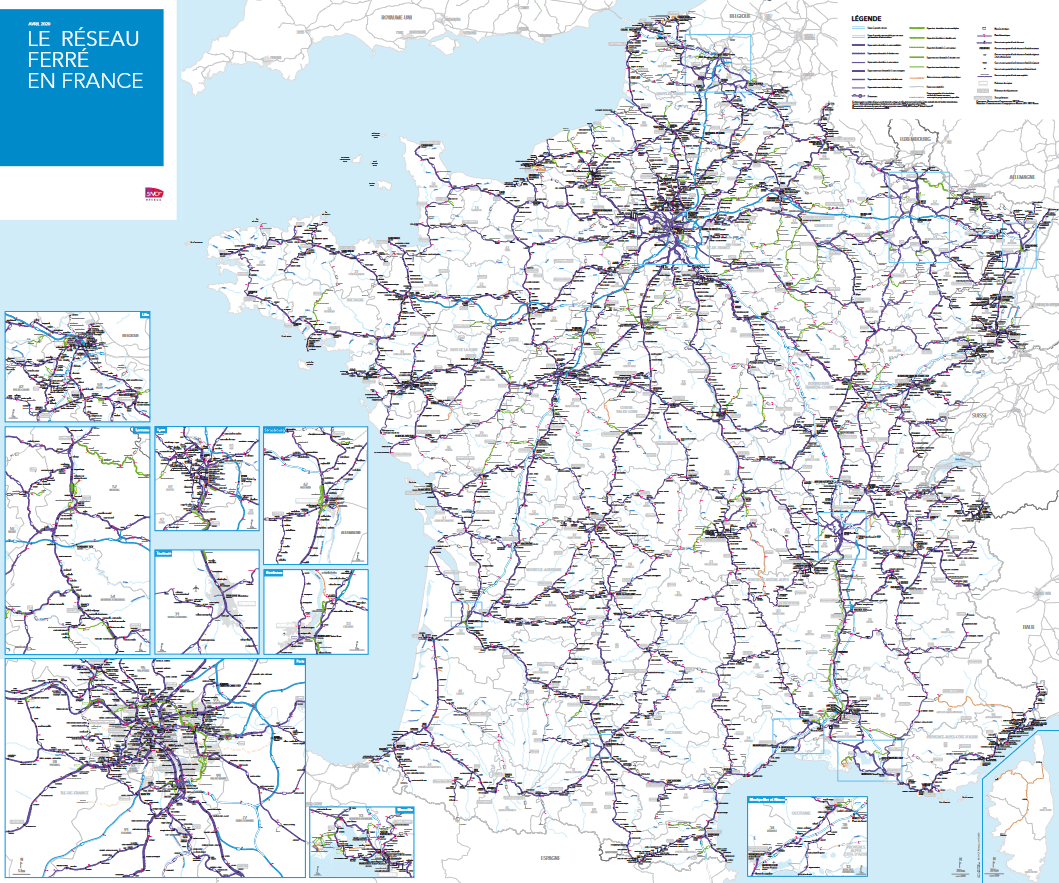
\includegraphics{images/carte-reseau-sncf-france2020.png} Figure 2.
Carte du réseau SNCF en France (2020)

Source :
\url{https://www.sncf-connect.com/aide/le-reseau-sncf-en-france-et-en-europe}

\hypertarget{voyageurs}{%
\section{Voyageurs}\label{voyageurs}}

Dans cette partie, nous étudierons les voyageurs. Afin de mieux
comprendre les voyageurs, nous avons choisi de nous intéresser aux
différents profils qui utilisent les trains des réseaux ferrés de
France.

\textbf{Visualisations réalisées}

\begin{enumerate}
\def\labelenumi{\arabic{enumi}.}
\item
  Nombre de voyageurs total par département (2022)
\item
  Répartition du nombre de voyageurs dans les gares d'un même
  département.Exemple département (77)
\item
  Explorer la répartition par âge des passagers
\item
  Catégorie socio professionnelle
\item
  Nombre de voyageurs par année
\end{enumerate}

Dans un premier temps, nous analysons le nombre de voyageurs par
département, pour nous intéresser ensuite à la proportion de voyageurs
dans les gares au sein d'un même département.

\emph{Le nombre de voyageurs est-il bien repartis entre les gares d'un
même département ?}

\hypertarget{nombre-de-voyageurs-total-par-duxe9partement-2022}{%
\subsection{1. Nombre de voyageurs total par département
(2022)}\label{nombre-de-voyageurs-total-par-duxe9partement-2022}}

\begin{Shaded}
\begin{Highlighting}[]
\NormalTok{freq\_departement }\OtherTok{\textless{}{-}}\NormalTok{ frequentation\_clean }\SpecialCharTok{\%\textgreater{}\%}
  \FunctionTok{filter}\NormalTok{(Année }\SpecialCharTok{==} \StringTok{"2022"}\NormalTok{)}

\NormalTok{freq\_departement }\OtherTok{\textless{}{-}}\NormalTok{ freq\_departement }\SpecialCharTok{\%\textgreater{}\%}
  \FunctionTok{group\_by}\NormalTok{(Département) }\SpecialCharTok{\%\textgreater{}\%}
  \FunctionTok{summarize}\NormalTok{(}\AttributeTok{Total\_passagers =} \FunctionTok{sum}\NormalTok{(Voyageurs))}

\FunctionTok{ggplot}\NormalTok{(freq\_departement, }\FunctionTok{aes}\NormalTok{(}\AttributeTok{x =}\NormalTok{ Total\_passagers, }\AttributeTok{y =}\NormalTok{ Département)) }\SpecialCharTok{+}
  \FunctionTok{geom\_bar}\NormalTok{(}\AttributeTok{stat =} \StringTok{"identity"}\NormalTok{) }\SpecialCharTok{+}
  \FunctionTok{labs}\NormalTok{(}\AttributeTok{title =} \StringTok{"Nombre de voyageurs total par département (2022)"}\NormalTok{,}
       \AttributeTok{subtitle =} \StringTok{"\textless{}Vue Globale\textgreater{}"}\NormalTok{,}
       \AttributeTok{x =} \StringTok{"Nombre total de passagers"}\NormalTok{,}
       \AttributeTok{y =} \StringTok{"Département"}\NormalTok{) }\SpecialCharTok{+}
  \FunctionTok{theme}\NormalTok{(}\AttributeTok{axis.text.y =} \FunctionTok{element\_text}\NormalTok{(}\AttributeTok{size =} \DecValTok{8}\NormalTok{))}
\end{Highlighting}
\end{Shaded}

\includegraphics{rogue-one_files/figure-latex/unnamed-chunk-6-1.pdf}

Comme le constat fait un peu plus haut, on observe que la région Ile de
France (composée des départements 75,77, 78, 91, 92, 93, 94) concentre
la plupart de la fréquentation. Ce constat est tout à fait correct étant
donné que la région concentre environ 12 millions de personnes.

On peut également créer une visualisation qui permettrait de connaitre
la fréquentation de chacune des régions.

\begin{Shaded}
\begin{Highlighting}[]
\FunctionTok{View}\NormalTok{(frequentation\_clean)}
\end{Highlighting}
\end{Shaded}

\hypertarget{ruxe9partition-du-nombre-de-voyageurs-dans-les-gares-dun-muxeame-duxe9partement.exemple-duxe9partement-77}{%
\subsection{2. Répartition du nombre de voyageurs dans les gares d'un
même département.Exemple département
(77)}\label{ruxe9partition-du-nombre-de-voyageurs-dans-les-gares-dun-muxeame-duxe9partement.exemple-duxe9partement-77}}

Grâce à cette visusalisation, on peut connaître les gares les plus
importantes en termes de fréquentation dans chacun des départements.

Dans le cas du département 77 et du premier jet de visualisation, on
observe que la gare de Melun est très fréquentée comparé aux autres
gares.

\begin{Shaded}
\begin{Highlighting}[]
\CommentTok{\#gares\_77 \textless{}{-} freq \%\textgreater{}\%}
\CommentTok{\#  filter(departement == "77")}

\CommentTok{\#ggplot(gares\_77, aes(x = Gare, y = Voyageurs)) +}
\CommentTok{\#  geom\_bar(stat = "identity") +}
\CommentTok{\#  labs(title = "Repartition des voyageurs dans les gares du département 77 en 2022",}
\CommentTok{\#       x = "Gare",}
\CommentTok{\#       y = "Nombre de passagers") +}
\CommentTok{\#  theme\_minimal() +}
\CommentTok{\#  theme(axis.text.x = element\_text(angle = 45, hjust = 1, size = 8))}
\end{Highlighting}
\end{Shaded}

Au sein du 77, on remarque des disparités entre les gares. Des gares
comme celle de Melun ou Chartrette concentre toute la fréquentation au
détriment de gares comme Bois-le-Roi.

On peut expliquer cela notamment après quelques recherches car en effet
le RER D désert Melun à la différence de petites gares comme celle de
Bois-le-Roi.

\textbf{Quel est le voyageur moyen de la SNCF ?}

\hypertarget{explorer-la-ruxe9partition-par-uxe2ge-des-passagers}{%
\subsection{3. Explorer la répartition par âge des
passagers}\label{explorer-la-ruxe9partition-par-uxe2ge-des-passagers}}

En raison de quelques problèmes dans l'ensemble de données, tels que des
codes UIC incohérents et des variations dans les années de recensement
et les données des stations, nous allons nous concentrer exclusivement
sur la répartition par âge pour les années 2015, 2016 et 2017.

Conserver les colonnes spécifiées dans frequentation et renommer Code
UIC en UIC et Filtrer le age\_voya pour une année 2015,16,17.

\begin{Shaded}
\begin{Highlighting}[]
\NormalTok{age\_filtered }\OtherTok{\textless{}{-}}\NormalTok{ age\_voya\_clean }\SpecialCharTok{\%\textgreater{}\%}
  \FunctionTok{select}\NormalTok{(}\SpecialCharTok{{-}}\NormalTok{Gare) }\SpecialCharTok{\%\textgreater{}\%}
  \FunctionTok{filter}\NormalTok{(Année }\SpecialCharTok{\%in\%} \FunctionTok{c}\NormalTok{(}\DecValTok{2015}\NormalTok{, }\DecValTok{2016}\NormalTok{, }\DecValTok{2017}\NormalTok{))}
\end{Highlighting}
\end{Shaded}

Filtrer freq\_selected par nom de station, en ne conservant que les
lignes qui correspondent à Nom dans age\_filtered, et vice versa.

\begin{Shaded}
\begin{Highlighting}[]
\NormalTok{joined\_dataset }\OtherTok{\textless{}{-}} \FunctionTok{inner\_join}\NormalTok{(age\_filtered, frequentation\_clean, }\FunctionTok{join\_by}\NormalTok{(UIC, Année))}
\NormalTok{cleaned\_dataset}\OtherTok{\textless{}{-}}\NormalTok{ joined\_dataset }\SpecialCharTok{\%\textgreater{}\%}
  \FunctionTok{pivot\_wider}\NormalTok{(}
    \AttributeTok{names\_from =} \StringTok{\textasciigrave{}}\AttributeTok{Classe d\textquotesingle{}âge}\StringTok{\textasciigrave{}}\NormalTok{, }
    \AttributeTok{values\_from =}\NormalTok{ Pourcentage, }
    \AttributeTok{values\_fill =} \FunctionTok{list}\NormalTok{(}\AttributeTok{Pourcentage =} \DecValTok{0}\NormalTok{)  }
\NormalTok{  )}
\end{Highlighting}
\end{Shaded}

Calculer le nombre de voyageurs dans chaque groupe d'âge et les nombre
total pour chaque année

\begin{Shaded}
\begin{Highlighting}[]
\NormalTok{age\_columns }\OtherTok{\textless{}{-}} \FunctionTok{c}\NormalTok{(}\StringTok{\textquotesingle{}19 ans et moins\textquotesingle{}}\NormalTok{, }\StringTok{\textquotesingle{}20 ans à 29 ans\textquotesingle{}}\NormalTok{, }\StringTok{\textquotesingle{}30 ans à 39 ans\textquotesingle{}}\NormalTok{, }\StringTok{\textquotesingle{}40 ans à 49 ans\textquotesingle{}}\NormalTok{, }\StringTok{\textquotesingle{}50 ans à 59 ans\textquotesingle{}}\NormalTok{, }\StringTok{\textquotesingle{}60 ans et plus\textquotesingle{}}\NormalTok{)}
\NormalTok{cleaned\_dataset }\OtherTok{\textless{}{-}}\NormalTok{ cleaned\_dataset }\SpecialCharTok{\%\textgreater{}\%}
  \FunctionTok{mutate}\NormalTok{(}\FunctionTok{across}\NormalTok{(}\FunctionTok{all\_of}\NormalTok{(age\_columns), }\SpecialCharTok{\textasciitilde{}}\NormalTok{ .x }\SpecialCharTok{*}\NormalTok{ Voyageurs }\SpecialCharTok{/} \DecValTok{100}\NormalTok{, }\AttributeTok{.names =} \StringTok{"passengers\_\{.col\}"}\NormalTok{))}
\NormalTok{age\_passenger\_totals }\OtherTok{\textless{}{-}}\NormalTok{ cleaned\_dataset }\SpecialCharTok{\%\textgreater{}\%}
  \FunctionTok{group\_by}\NormalTok{(Année) }\SpecialCharTok{\%\textgreater{}\%}
  \FunctionTok{summarise}\NormalTok{(}\FunctionTok{across}\NormalTok{(}\FunctionTok{starts\_with}\NormalTok{(}\StringTok{"passengers"}\NormalTok{), sum, }\AttributeTok{.names =} \StringTok{"total\_\{.col\}"}\NormalTok{))}
\end{Highlighting}
\end{Shaded}

L'étape suivante consiste à calculer le pourcentage des groupes d'âge
ainsi que la cartographie.

\begin{Shaded}
\begin{Highlighting}[]
\NormalTok{age\_passenger\_totals\_long }\OtherTok{\textless{}{-}}\NormalTok{ age\_passenger\_totals }\SpecialCharTok{\%\textgreater{}\%}
  \FunctionTok{pivot\_longer}\NormalTok{(}
    \AttributeTok{cols =} \FunctionTok{starts\_with}\NormalTok{(}\StringTok{"total\_passengers"}\NormalTok{),}
    \AttributeTok{names\_to =} \StringTok{"Age\_Group"}\NormalTok{,}
    \AttributeTok{values\_to =} \StringTok{"Total\_Passengers"}\NormalTok{,}
    \AttributeTok{names\_prefix =} \StringTok{"total\_passengers\_"}
\NormalTok{  )}
\NormalTok{age\_passenger\_totals\_long }\OtherTok{\textless{}{-}}\NormalTok{ age\_passenger\_totals\_long }\SpecialCharTok{\%\textgreater{}\%}
  \FunctionTok{group\_by}\NormalTok{(Année) }\SpecialCharTok{\%\textgreater{}\%}
  \FunctionTok{mutate}\NormalTok{(}\AttributeTok{Total\_Passengers\_Year =} \FunctionTok{sum}\NormalTok{(Total\_Passengers)) }\SpecialCharTok{\%\textgreater{}\%}
  \FunctionTok{ungroup}\NormalTok{() }\SpecialCharTok{\%\textgreater{}\%}
  \FunctionTok{mutate}\NormalTok{(}\AttributeTok{Percentage =}\NormalTok{ (Total\_Passengers }\SpecialCharTok{/}\NormalTok{ Total\_Passengers\_Year) }\SpecialCharTok{*} \DecValTok{100}\NormalTok{)}
\FunctionTok{ggplot}\NormalTok{(age\_passenger\_totals\_long, }\FunctionTok{aes}\NormalTok{(}\AttributeTok{x =}\NormalTok{ Année, }\AttributeTok{y =}\NormalTok{ Percentage, }\AttributeTok{fill =}\NormalTok{ Age\_Group)) }\SpecialCharTok{+}
  \FunctionTok{geom\_bar}\NormalTok{(}\AttributeTok{stat =} \StringTok{"identity"}\NormalTok{, }\AttributeTok{position =} \StringTok{"dodge"}\NormalTok{) }\SpecialCharTok{+}
  \FunctionTok{labs}\NormalTok{(}\AttributeTok{title =} \StringTok{"Pourcentage de passagers par groupe d\textquotesingle{}âge et année"}\NormalTok{,}
       \AttributeTok{x =} \StringTok{"Année"}\NormalTok{,}
       \AttributeTok{y =} \StringTok{"Pourcentage (\%)"}\NormalTok{,}
       \AttributeTok{fill =} \StringTok{"Groupes d\textquotesingle{}âge"}\NormalTok{) }\SpecialCharTok{+}
  \FunctionTok{theme\_minimal}\NormalTok{()}
\end{Highlighting}
\end{Shaded}

\includegraphics{rogue-one_files/figure-latex/unnamed-chunk-12-1.pdf}

\hypertarget{catuxe9gorie-socio-professionnelle}{%
\subsection{4. Catégorie socio
professionnelle}\label{catuxe9gorie-socio-professionnelle}}

Il est également intéressant de recueillir des informations sur le
voyageur moyen de la SNCF, En premier lieu nous allons voir les
différentes catégories socio professionnelles.

PS : Le Pourcentage correspond au pourcentage par rapport au CSP d'une
gare.

\begin{Shaded}
\begin{Highlighting}[]
\NormalTok{profil\_moyen }\OtherTok{\textless{}{-}}\NormalTok{ CSP\_voya }\SpecialCharTok{\%\textgreater{}\%}
  \FunctionTok{group\_by}\NormalTok{(CSP) }\SpecialCharTok{\%\textgreater{}\%}
  \FunctionTok{summarise}\NormalTok{(}\AttributeTok{Pourcentage\_moyen =} \FunctionTok{mean}\NormalTok{(Pourcentage, }\AttributeTok{na.rm =} \ConstantTok{TRUE}\NormalTok{))}

\NormalTok{profil\_moyen }\OtherTok{\textless{}{-}}\NormalTok{ profil\_moyen }\SpecialCharTok{\%\textgreater{}\%}
  \FunctionTok{arrange}\NormalTok{(}\FunctionTok{desc}\NormalTok{(Pourcentage\_moyen))}
\NormalTok{profil\_moyen}
\end{Highlighting}
\end{Shaded}

\begin{verbatim}
## # A tibble: 13 x 2
##    CSP                                                         Pourcentage_moyen
##    <chr>                                                                   <dbl>
##  1 Ouvrier, Employé                                                       21.3  
##  2 Cadre, Profession libérale ou intellectuelle, Chef d'entre~            20.1  
##  3 Non communiqué                                                         17.9  
##  4 Etudiant (après le bac)                                                15.5  
##  5 Retraité                                                               11.3  
##  6 Scolaire (avant le bac)                                                 5.95 
##  7 Technicien, Agent de maîtrise                                           5.41 
##  8 Sans emploi                                                             5.04 
##  9 Enseignant, Professeur                                                  3.78 
## 10 Artisan, Commerçant, Chef d'entreprise TPE                              3.40 
## 11 Autre                                                                   2.31 
## 12 Militaire                                                               1.29 
## 13 Agriculteur, Exploitant agricole                                        0.415
\end{verbatim}

Regroupement des CSP par pourcentages.

\begin{Shaded}
\begin{Highlighting}[]
\FunctionTok{ggplot}\NormalTok{(profil\_moyen, }\FunctionTok{aes}\NormalTok{(}\AttributeTok{x =} \FunctionTok{reorder}\NormalTok{(CSP, }\SpecialCharTok{{-}}\NormalTok{Pourcentage\_moyen), }\AttributeTok{y =}\NormalTok{ Pourcentage\_moyen)) }\SpecialCharTok{+}
  \FunctionTok{geom\_bar}\NormalTok{(}\AttributeTok{stat =} \StringTok{"identity"}\NormalTok{) }\SpecialCharTok{+}
  \FunctionTok{coord\_flip}\NormalTok{() }\SpecialCharTok{+} 
  \FunctionTok{labs}\NormalTok{(}\AttributeTok{title =} \StringTok{"Profil Moyen du Voyageur SNCF par CSP"}\NormalTok{,}
       \AttributeTok{x =} \StringTok{"Catégorie Socio{-}Professionnelle"}\NormalTok{,}
       \AttributeTok{y =} \StringTok{"Pourcentage Moyen"}\NormalTok{) }\SpecialCharTok{+}
  \FunctionTok{theme\_minimal}\NormalTok{()}
\end{Highlighting}
\end{Shaded}

\includegraphics{rogue-one_files/figure-latex/unnamed-chunk-14-1.pdf}

\hypertarget{nombre-de-voyageurs-par-annuxe9e}{%
\subsection{5. Nombre de voyageurs par
année}\label{nombre-de-voyageurs-par-annuxe9e}}

Réalisons un graphique simple qui nous montre le nombre de voyageurs
total par année.

Apercu du dataset fréquentations

\begin{Shaded}
\begin{Highlighting}[]
\FunctionTok{head}\NormalTok{(frequentation)}
\end{Highlighting}
\end{Shaded}

\begin{verbatim}
## # A tibble: 6 x 20
##   `Nom de la gare`      `Code UIC` `Code postal` `Segmentation DRG`
##   <chr>                      <dbl>         <dbl> <chr>             
## 1 Abbaretz                87481614         44170 C                 
## 2 Ablon-sur-Seine         87545269         94480 B                 
## 3 Achères Grand Cormier   87386052         78100 B                 
## 4 Acheux - Franleu        87316745         80560 C                 
## 5 Aigrefeuille le Thou    87485193         17290 C                 
## 6 Aigueperse              87734129         63260 C                 
## # i 16 more variables: `Total Voyageurs 2022` <dbl>,
## #   `Total Voyageurs + Non voyageurs 2022` <dbl>, `Total Voyageurs 2021` <dbl>,
## #   `Total Voyageurs + Non voyageurs 2021` <dbl>, `Total Voyageurs 2020` <dbl>,
## #   `Total Voyageurs + Non voyageurs 2020` <dbl>, `Total Voyageurs 2019` <dbl>,
## #   `Total Voyageurs + Non voyageurs 2019` <dbl>, `Total Voyageurs 2018` <dbl>,
## #   `Total Voyageurs + Non voyageurs 2018` <dbl>, `Total Voyageurs 2017` <dbl>,
## #   `Total Voyageurs + Non voyageurs 2017` <dbl>, ...
\end{verbatim}

\begin{Shaded}
\begin{Highlighting}[]
\CommentTok{\#total\_par\_annee \textless{}{-} frequentation \%\textgreater{}\%}
\CommentTok{\#  summarise(}
\CommentTok{\#    Total\_2022 = sum(\textasciigrave{}passagers2022\textasciigrave{}, na.rm = TRUE),}
\CommentTok{\#    Total\_2021 = sum(\textasciigrave{}Total Voyageurs 2021\textasciigrave{}, na.rm = TRUE),}
\CommentTok{\#    Total\_2020 = sum(\textasciigrave{}Total Voyageurs 2020\textasciigrave{}, na.rm = TRUE),}
\CommentTok{\#    Total\_2019 = sum(\textasciigrave{}Total Voyageurs 2019\textasciigrave{}, na.rm = TRUE),}
\CommentTok{\#    Total\_2018 = sum(\textasciigrave{}Total Voyageurs 2018\textasciigrave{}, na.rm = TRUE),}
\CommentTok{\#    Total\_2017 = sum(\textasciigrave{}Total Voyageurs 2017\textasciigrave{}, na.rm = TRUE),}
\CommentTok{\#    Total\_2016 = sum(\textasciigrave{}Total Voyageurs 2016\textasciigrave{}, na.rm = TRUE),}
\CommentTok{\#    Total\_2015 = sum(\textasciigrave{}Total Voyageurs 2015\textasciigrave{}, na.rm = TRUE)}
\CommentTok{\#  )}

\CommentTok{\#data\_long \textless{}{-} pivot\_longer(total\_par\_annee, cols = everything(), names\_to = "Annee", values\_to = "Total")}

\CommentTok{\#ggplot(data\_long, aes(x = Annee, y = Total, group = 1)) +}
\CommentTok{\#  geom\_line() +  }
\CommentTok{\#  geom\_point() +  }
\CommentTok{\#  labs(title = "Nombre total de voyageurs par année",}
\CommentTok{\#       x = "Année",}
\CommentTok{\#       y = "Nombre total de voyageurs") +}
\CommentTok{\#  theme\_minimal()}
\end{Highlighting}
\end{Shaded}

On voit rapidement qu'il y a un ``trou'' du à la période COVID 2020.

Maintenant intéressons nous aux nombres de voyageurs par segmentation
DRG.

\begin{Shaded}
\begin{Highlighting}[]
\CommentTok{\#data\_segmentation \textless{}{-} frequentation \%\textgreater{}\%}
\CommentTok{\#  group\_by(\textasciigrave{}Segmentation DRG\textasciigrave{}) \%\textgreater{}\%}
\CommentTok{\#  summarise(Total\_2022 = sum(\textasciigrave{}passagers2022\textasciigrave{}, na.rm = TRUE)) \%\textgreater{}\%}
\CommentTok{\#  na.omit()}
\CommentTok{\#head(data\_segmentation)}

\CommentTok{\#ggplot(data\_segmentation, aes(x = \textasciigrave{}Segmentation DRG\textasciigrave{}, y = Total\_2022, fill = \textasciigrave{}Segmentation DRG\textasciigrave{})) +}
\CommentTok{\#  geom\_bar(stat = "identity") +}
\CommentTok{\#  labs(title = "Répartition des voyageurs par segmentation DRG en 2022",}
\CommentTok{\#       x = "Segmentation DRG",}
\CommentTok{\#       y = "Nombre total de voyageurs") +}
\CommentTok{\#  theme\_minimal()}
\end{Highlighting}
\end{Shaded}

\hypertarget{objets}{%
\section{Objets}\label{objets}}

Dans cette partie, nous voulons nous intéresser plus particulièrement
aux objets.

\textbf{Visualisations réalisées}

\begin{enumerate}
\def\labelenumi{\arabic{enumi}.}
\item
  Objets perdus
\item
  Objets restitués
\item
  Probabilité de retrouver un objet perdu
\item
  Probabilité de retrouver un objet selon son type
\end{enumerate}

\hypertarget{objets-perdus}{%
\subsection{1. Objets perdus}\label{objets-perdus}}

Tout d'abord, petite visualisation du dataset obj\_perdus

\begin{Shaded}
\begin{Highlighting}[]
\FunctionTok{head}\NormalTok{(obj\_perdus)}
\end{Highlighting}
\end{Shaded}

\begin{verbatim}
## # A tibble: 6 x 6
##   Date de la déclaration de~1 Gare  `Code UIC` `Nature d'objets` `Type d'objets`
##   <dttm>                      <chr> <chr>      <chr>             <chr>          
## 1 2019-05-24 16:52:18         Pari~ 0087113001 Manteau, veste, ~ Vêtements, cha~
## 2 2019-05-24 16:53:32         <NA>  <NA>       Téléphone portab~ Appareils élec~
## 3 2019-05-24 17:00:58         <NA>  <NA>       Sac de voyage, s~ Bagagerie: sac~
## 4 2019-05-24 17:09:28         <NA>  <NA>       Autre pièce ou p~ Pièces d'ident~
## 5 2019-05-24 17:11:10         Pari~ 0087384008 Sacoche ventrale~ Bagagerie: sac~
## 6 2019-05-24 17:30:25         <NA>  <NA>       Téléphone portab~ Appareils élec~
## # i abbreviated name: 1: `Date de la déclaration de perte`
## # i 1 more variable: `Type d'enregistrement` <chr>
\end{verbatim}

\begin{Shaded}
\begin{Highlighting}[]
\FunctionTok{summary}\NormalTok{(obj\_perdus)}
\end{Highlighting}
\end{Shaded}

\begin{verbatim}
##  Date de la déclaration de perte      Gare             Code UIC        
##  Min.   :2013-05-24 11:02:10.00   Length:1876131     Length:1876131    
##  1st Qu.:2016-12-08 06:49:31.50   Class :character   Class :character  
##  Median :2019-06-21 06:06:05.00   Mode  :character   Mode  :character  
##  Mean   :2019-07-22 20:41:06.14                                        
##  3rd Qu.:2022-05-30 09:10:26.00                                        
##  Max.   :2024-04-30 09:00:10.00                                        
##  Nature d'objets    Type d'objets      Type d'enregistrement
##  Length:1876131     Length:1876131     Length:1876131       
##  Class :character   Class :character   Class :character     
##  Mode  :character   Mode  :character   Mode  :character     
##                                                             
##                                                             
## 
\end{verbatim}

Quelque chose m'interpelle dès le début : c'est la colonne ``Type
d'enregistrement'', il semble que celle-ci est toujours remplie de la
même manière

\begin{Shaded}
\begin{Highlighting}[]
\NormalTok{enregistrement }\OtherTok{\textless{}{-}}\NormalTok{ obj\_perdus }\SpecialCharTok{\%\textgreater{}\%}
  \FunctionTok{select}\NormalTok{(}\AttributeTok{en =} \StringTok{\textasciigrave{}}\AttributeTok{Type d\textquotesingle{}enregistrement}\StringTok{\textasciigrave{}}\NormalTok{)}
\NormalTok{diff\_enre }\OtherTok{\textless{}{-}} \FunctionTok{n\_distinct}\NormalTok{(enregistrement)}
\end{Highlighting}
\end{Shaded}

C'est donc le cas, donc nous n'utiliserons pas cette colonne .

On distingue aussi que de nombreuses gares ne sont pas présentes.

Nous voulons effectuer plusieurs réductions sur ce jeu de données. Tout
d'abord, les informations que nous avons datent de 2019 jusqu'à nos
jours. Si nous voulons faire des recoupements avec le dataset de
voyageur, nous allons restreindre les dates à 2019 seulement car les
années 2020 et 2021 ne sont pas forcément représentatives du traffic
ferroviaire normal. L'année 2022 sera analysée prochainement pour voir
si une tendance peut commencer à apparaître.

\begin{Shaded}
\begin{Highlighting}[]
\NormalTok{obj\_perdus\_2019 }\OtherTok{\textless{}{-}}\NormalTok{ obj\_perdus }\SpecialCharTok{\%\textgreater{}\%}
  \FunctionTok{select}\NormalTok{(}\AttributeTok{date =} \StringTok{\textasciigrave{}}\AttributeTok{Date de la déclaration de perte}\StringTok{\textasciigrave{}}\NormalTok{, }\AttributeTok{gare =} \StringTok{"Gare"}\NormalTok{, }\AttributeTok{UIC =} \StringTok{"Code UIC"}\NormalTok{, }\AttributeTok{nature =} \StringTok{"Nature d\textquotesingle{}objets"}\NormalTok{, }\AttributeTok{type =} \StringTok{"Type d\textquotesingle{}objets"}\NormalTok{) }\SpecialCharTok{\%\textgreater{}\%}
  \FunctionTok{filter}\NormalTok{(date }\SpecialCharTok{\textless{}} \FunctionTok{ymd}\NormalTok{(}\DecValTok{20200101}\NormalTok{)) }\SpecialCharTok{\%\textgreater{}\%} 
  \FunctionTok{filter}\NormalTok{(date }\SpecialCharTok{\textgreater{}} \FunctionTok{ymd}\NormalTok{(}\DecValTok{20190101}\NormalTok{))}
\FunctionTok{count}\NormalTok{(obj\_perdus\_2019)}
\end{Highlighting}
\end{Shaded}

\begin{verbatim}
## # A tibble: 1 x 1
##        n
##    <int>
## 1 185065
\end{verbatim}

Nous avons donc maintenant 185 065 entrées dans notre dataframe.

Découvrons ce que celui-ci nous cache dans la répartition des objets
perdus :

\begin{Shaded}
\begin{Highlighting}[]
\NormalTok{obj\_perdus\_2019 }\SpecialCharTok{\%\textgreater{}\%} 
  \FunctionTok{ggplot}\NormalTok{(}\FunctionTok{aes}\NormalTok{(}\AttributeTok{y=}\FunctionTok{fct\_rev}\NormalTok{(}\FunctionTok{fct\_infreq}\NormalTok{(type)))) }\SpecialCharTok{+}
  \FunctionTok{geom\_bar}\NormalTok{() }\SpecialCharTok{+}
  \FunctionTok{labs}\NormalTok{(}\AttributeTok{title =} \StringTok{"Nombre d\textquotesingle{}objets perdus par type d\textquotesingle{}objets en 2019"}\NormalTok{,}
       \AttributeTok{y =} \StringTok{"Type d\textquotesingle{}objet"}\NormalTok{,}
       \AttributeTok{x =} \StringTok{"Nombre d\textquotesingle{}objets perdus en unité"}\NormalTok{)}\SpecialCharTok{+}
  \FunctionTok{theme\_minimal}\NormalTok{() }\SpecialCharTok{+}
  \FunctionTok{theme}\NormalTok{(}\AttributeTok{axis.text.y =} \FunctionTok{element\_text}\NormalTok{(}\AttributeTok{size =} \FunctionTok{rel}\NormalTok{(}\FloatTok{0.8}\NormalTok{)))}
\end{Highlighting}
\end{Shaded}

\includegraphics{rogue-one_files/figure-latex/unnamed-chunk-21-1.pdf}

Sans surprise, les objets les plus couramment perdus sont donc dans
l'ordre :

\begin{itemize}
\item
  Bagages
\item
  Appareils électroniques
\item
  Vêtements
\end{itemize}

\begin{Shaded}
\begin{Highlighting}[]
\NormalTok{obj\_perdus\_trouves }\OtherTok{\textless{}{-}}\NormalTok{ obj\_perdus\_2019 }\SpecialCharTok{\%\textgreater{}\%}
  \FunctionTok{filter}\NormalTok{(}\FunctionTok{is.na}\NormalTok{(gare) }\SpecialCharTok{==} \ConstantTok{FALSE}\NormalTok{)}

\FunctionTok{count}\NormalTok{(obj\_perdus\_trouves)}
\end{Highlighting}
\end{Shaded}

\begin{verbatim}
## # A tibble: 1 x 1
##       n
##   <int>
## 1 54834
\end{verbatim}

\begin{Shaded}
\begin{Highlighting}[]
\NormalTok{obj\_perdus\_trouves }\SpecialCharTok{\%\textgreater{}\%} 
  \FunctionTok{ggplot}\NormalTok{(}\FunctionTok{aes}\NormalTok{(}\AttributeTok{y=}\FunctionTok{fct\_rev}\NormalTok{(}\FunctionTok{fct\_infreq}\NormalTok{(type)))) }\SpecialCharTok{+}
  \FunctionTok{geom\_bar}\NormalTok{() }\SpecialCharTok{+}
  \FunctionTok{labs}\NormalTok{(}\AttributeTok{title =} \StringTok{"Nombre d\textquotesingle{}objets perdus retrouvés par type d\textquotesingle{}objets en 2019"}\NormalTok{,}
       \AttributeTok{y =} \StringTok{"Type d\textquotesingle{}objet"}\NormalTok{,}
       \AttributeTok{x =} \StringTok{"Nombre d\textquotesingle{}objets perdus en unité"}\NormalTok{) }\SpecialCharTok{+}
  \FunctionTok{theme\_minimal}\NormalTok{() }\SpecialCharTok{+}
  \FunctionTok{theme}\NormalTok{(}\AttributeTok{axis.text.y =} \FunctionTok{element\_text}\NormalTok{(}\AttributeTok{size =} \FunctionTok{rel}\NormalTok{(}\FloatTok{0.8}\NormalTok{)))}
\end{Highlighting}
\end{Shaded}

\includegraphics{rogue-one_files/figure-latex/unnamed-chunk-23-1.pdf}

\hypertarget{objets-restituuxe9s}{%
\subsection{2. Objets restitués}\label{objets-restituuxe9s}}

Nous allons ensuite parcourir le dataset 7 : obj\_trouves

\begin{Shaded}
\begin{Highlighting}[]
\NormalTok{obj\_trouves\_2019 }\OtherTok{\textless{}{-}}\NormalTok{ obj\_trouves }\SpecialCharTok{\%\textgreater{}\%}
  \FunctionTok{select}\NormalTok{(}\AttributeTok{date =} \StringTok{\textasciigrave{}}\AttributeTok{Date}\StringTok{\textasciigrave{}}\NormalTok{,}\AttributeTok{restitution =} \StringTok{\textasciigrave{}}\AttributeTok{Date et heure de restitution}\StringTok{\textasciigrave{}}\NormalTok{ ,}\AttributeTok{gare =} \StringTok{"Gare"}\NormalTok{, }\AttributeTok{UIC =} \StringTok{"Code UIC"}\NormalTok{, }\AttributeTok{nature =} \StringTok{"Nature d\textquotesingle{}objets"}\NormalTok{, }\AttributeTok{type =} \StringTok{"Type d\textquotesingle{}objets"}\NormalTok{) }\SpecialCharTok{\%\textgreater{}\%}
  \FunctionTok{filter}\NormalTok{(date }\SpecialCharTok{\textless{}} \FunctionTok{ymd}\NormalTok{(}\DecValTok{20200101}\NormalTok{)) }\SpecialCharTok{\%\textgreater{}\%} 
  \FunctionTok{filter}\NormalTok{(date }\SpecialCharTok{\textgreater{}} \FunctionTok{ymd}\NormalTok{(}\DecValTok{20190101}\NormalTok{))}
\FunctionTok{count}\NormalTok{(obj\_trouves\_2019)}
\end{Highlighting}
\end{Shaded}

\begin{verbatim}
## # A tibble: 1 x 1
##       n
##   <int>
## 1 88258
\end{verbatim}

On découvre donc qu'il y a plus d'objets trouvés que d'objets perdus
rendus. Cela veut donc dire que tous les objets récupérés ne sont pas
forcément déclarés comme perdus au préalable.

\begin{Shaded}
\begin{Highlighting}[]
\NormalTok{obj\_trouves\_rendus }\OtherTok{\textless{}{-}}\NormalTok{ obj\_trouves\_2019 }\SpecialCharTok{\%\textgreater{}\%}
  \FunctionTok{filter}\NormalTok{(}\FunctionTok{is.na}\NormalTok{(UIC) }\SpecialCharTok{==} \ConstantTok{FALSE}\NormalTok{)}

\FunctionTok{count}\NormalTok{(obj\_trouves\_rendus)}
\end{Highlighting}
\end{Shaded}

\begin{verbatim}
## # A tibble: 1 x 1
##       n
##   <int>
## 1 88239
\end{verbatim}

On voit qu'il y a 19 objets rendus qui n'ont pas été identifiés par des
code UIC ce qui est étrange. Voyons cela de plus près :

\begin{Shaded}
\begin{Highlighting}[]
\NormalTok{obj\_trouves\_sans\_UIC }\OtherTok{\textless{}{-}}\NormalTok{ obj\_trouves\_2019 }\SpecialCharTok{\%\textgreater{}\%}
  \FunctionTok{filter}\NormalTok{(}\FunctionTok{is.na}\NormalTok{(UIC) }\SpecialCharTok{==} \ConstantTok{TRUE}\NormalTok{)}

\NormalTok{obj\_trouves\_sans\_UIC}
\end{Highlighting}
\end{Shaded}

\begin{verbatim}
## # A tibble: 19 x 6
##    date                restitution         gare  UIC   nature              type 
##    <dttm>              <dttm>              <chr> <chr> <chr>               <chr>
##  1 2019-11-27 18:51:31 NA                  <NA>  <NA>  Sac d'enseigne (pl~ Baga~
##  2 2019-12-18 12:09:32 NA                  <NA>  <NA>  Sac à dos           Baga~
##  3 2019-12-19 10:17:09 NA                  <NA>  <NA>  Autre pièce ou pap~ Pièc~
##  4 2019-08-26 07:49:55 NA                  <NA>  <NA>  Téléphone portable  Appa~
##  5 2019-08-27 09:01:52 NA                  <NA>  <NA>  Porte-monnaie, por~ Port~
##  6 2019-09-03 18:58:21 NA                  <NA>  <NA>  Sac de voyage, sac~ Baga~
##  7 2019-08-22 16:20:41 NA                  <NA>  <NA>  Carte d'identité, ~ Pièc~
##  8 2019-08-31 08:48:21 2021-01-06 06:14:46 <NA>  <NA>  Valise, sac sur ro~ Baga~
##  9 2019-03-05 07:14:37 NA                  <NA>  <NA>  Carte d'identité, ~ Pièc~
## 10 2019-09-02 17:16:33 NA                  <NA>  <NA>  Téléphone portable~ Appa~
## 11 2019-09-04 11:28:10 2019-09-05 15:49:33 <NA>  <NA>  Téléphone portable  Appa~
## 12 2019-05-06 12:35:54 2019-05-07 08:15:26 <NA>  <NA>  Sac à dos           Baga~
## 13 2019-12-17 14:52:16 2020-01-14 11:48:42 <NA>  <NA>  Sac de voyage, sac~ Baga~
## 14 2019-11-27 19:10:10 NA                  <NA>  <NA>  Sac d'enseigne (pl~ Baga~
## 15 2019-12-02 14:28:36 NA                  <NA>  <NA>  Autres divers       Dive~
## 16 2019-09-03 18:54:07 NA                  <NA>  <NA>  Valise, sac sur ro~ Baga~
## 17 2019-09-04 17:15:19 NA                  <NA>  <NA>  Carte de crédit     Port~
## 18 2019-12-18 12:02:47 NA                  <NA>  <NA>  Carte d'identité, ~ Pièc~
## 19 2019-09-17 16:38:07 NA                  <NA>  <NA>  Valise, sac sur ro~ Baga~
\end{verbatim}

En voyant que la gare n'est pas présente non plus, on peut juger ce
rendu comme ayant été entré dans la database sans qu'il n'ait été rendu
dans une gare. On peut supposer un rendu dans le train juste après la
perte.

Nous allons maintenant essayer de comprendre ce qu'est ce code UIC et
s'il y a une relation entre les codes UIC des pertes et des objets
trouvés.

Nous allons donc comparer les 2 listes de code UIC

\begin{Shaded}
\begin{Highlighting}[]
\NormalTok{liste\_UIC\_perdus }\OtherTok{\textless{}{-}}\NormalTok{ obj\_perdus\_trouves }\SpecialCharTok{\%\textgreater{}\%}
  \FunctionTok{select}\NormalTok{(UIC)}
\NormalTok{liste\_UIC\_trouves }\OtherTok{\textless{}{-}}\NormalTok{ obj\_trouves\_rendus }\SpecialCharTok{\%\textgreater{}\%}
  \FunctionTok{select}\NormalTok{(UIC)}
\FunctionTok{count}\NormalTok{(}\FunctionTok{intersect}\NormalTok{(liste\_UIC\_perdus, liste\_UIC\_trouves))}
\end{Highlighting}
\end{Shaded}

\begin{verbatim}
## # A tibble: 1 x 1
##       n
##   <int>
## 1   145
\end{verbatim}

\begin{Shaded}
\begin{Highlighting}[]
\FunctionTok{count}\NormalTok{(}\FunctionTok{setdiff}\NormalTok{(liste\_UIC\_perdus,liste\_UIC\_trouves))}
\end{Highlighting}
\end{Shaded}

\begin{verbatim}
## # A tibble: 1 x 1
##       n
##   <int>
## 1     1
\end{verbatim}

Il semble que seulement 146 code UIC différents et après quelques
recherches en ligne, le code UIC est l'ID des gares. Donc cette colonne
ne nous est pas forcément utile.

Nous allons donc maintenant essayer de mettre en relation plutôt les
dates entre les 2 datasets :

\begin{Shaded}
\begin{Highlighting}[]
\NormalTok{liste\_date\_perdus }\OtherTok{\textless{}{-}}\NormalTok{ obj\_perdus\_trouves }\SpecialCharTok{\%\textgreater{}\%}
  \FunctionTok{select}\NormalTok{(date)}
\NormalTok{liste\_date\_trouves }\OtherTok{\textless{}{-}}\NormalTok{ obj\_trouves\_rendus }\SpecialCharTok{\%\textgreater{}\%}
  \FunctionTok{select}\NormalTok{(date)}
\FunctionTok{intersect}\NormalTok{(liste\_date\_perdus, liste\_date\_trouves)}
\end{Highlighting}
\end{Shaded}

\begin{verbatim}
## # A tibble: 302 x 1
##    date               
##    <dttm>             
##  1 2019-02-02 13:52:46
##  2 2019-02-04 11:01:06
##  3 2019-02-11 11:25:20
##  4 2019-02-11 16:54:56
##  5 2019-10-02 08:35:47
##  6 2019-01-30 15:21:08
##  7 2019-10-04 14:48:42
##  8 2019-10-10 10:14:01
##  9 2019-03-06 14:04:44
## 10 2019-01-07 10:16:07
## # i 292 more rows
\end{verbatim}

\begin{Shaded}
\begin{Highlighting}[]
\FunctionTok{setdiff}\NormalTok{(liste\_date\_perdus,liste\_date\_trouves)}
\end{Highlighting}
\end{Shaded}

\begin{verbatim}
## # A tibble: 54,429 x 1
##    date               
##    <dttm>             
##  1 2019-05-24 16:52:18
##  2 2019-05-24 17:11:10
##  3 2019-05-24 18:26:47
##  4 2019-05-24 19:29:14
##  5 2019-05-24 19:58:27
##  6 2019-05-25 07:41:26
##  7 2019-05-25 07:53:09
##  8 2019-05-25 08:09:59
##  9 2019-05-25 08:16:59
## 10 2019-05-25 08:45:00
## # i 54,419 more rows
\end{verbatim}

Nous avons donc seulement 302 dates en commun entre les 2 jeux de
données ce qui est très faible. On peut donc supposer que les 2 datasets
ne sont pas liés et les dates ne correspondent pas. On peut supposer que
la date des objets perdus provient du questionnaire de perte que les
voyageurs remplissent, tandis que la date des objets trouvés provient du
formulaire remplit par les agents SNCF.

Nous ne pouvons donc pas faire de relation directe entre un objet
déclaré comme perdu et un objet déclaré comme trouvé.

Il est donc difficile de faire des hypothèses très spécifique sur les
probabilités de retrouver un objet perdu. La façon de faire ça serait de
connaître un nombre précis de pertes et sur ces pertes savoir combien
d'entre elles ont été rendues. Sans le lien entre les pertes et les
objets rendus, énormément de biais peuvent apparaître. Pour faire les
prochaines probabilités, nous allons faire l'hypothèse que l'ensemble
des objets rendus ont fait l'objet d'une entrée dans le formulaire de
perte.

\textbf{Quelles sont les chances de retrouver un objet perdu ?}

\hypertarget{probabilituxe9-de-retrouver-un-objet-perdu}{%
\subsection{3. Probabilité de retrouver un objet
perdu}\label{probabilituxe9-de-retrouver-un-objet-perdu}}

Pour cette première probabilité nous allons faire un calcul simple :

(Nombre d'objets retrouvés / Nombre d'objets perdus) *100

Cela s'exprime ainsi :

\begin{Shaded}
\begin{Highlighting}[]
\NormalTok{proba\_commune }\OtherTok{\textless{}{-}}\NormalTok{ (}\FunctionTok{count}\NormalTok{(obj\_trouves\_2019) }\SpecialCharTok{/} \FunctionTok{count}\NormalTok{(obj\_perdus\_2019) }\SpecialCharTok{*} \DecValTok{100}\NormalTok{)}
\NormalTok{proba\_commune}
\end{Highlighting}
\end{Shaded}

\begin{verbatim}
##          n
## 1 47.69027
\end{verbatim}

Je trouve la probabilité relativement élevée car pas très éloignée du
50\%. Peut-être aussi que le postulat personnel avant le calcul était
relativement pessimiste.

\textbf{Quelles sont les chances de retrouver un objet en fonction de
son type ?}

\hypertarget{probabilituxe9-de-retrouver-un-objet-selon-son-type}{%
\subsection{4. Probabilité de retrouver un objet selon son
type}\label{probabilituxe9-de-retrouver-un-objet-selon-son-type}}

Afin d'avoir une probabilité selon le type il faut donc que nous
effectuons la même opération que précédemment avec comme paramètre le
type de l'objet.

N.B. la ``nature'' dans l'intitulé de la question a été changé en type
car la nature entrée dans le formulaire des objets trouvés est trop
spécifique.

\begin{Shaded}
\begin{Highlighting}[]
\NormalTok{type\_obj\_perdus }\OtherTok{\textless{}{-}}\NormalTok{ obj\_perdus\_2019 }\SpecialCharTok{\%\textgreater{}\%}
  \FunctionTok{select}\NormalTok{(type)}
\NormalTok{type\_obj\_trouves }\OtherTok{\textless{}{-}}\NormalTok{ obj\_trouves\_2019 }\SpecialCharTok{\%\textgreater{}\%}
  \FunctionTok{select}\NormalTok{(type)}
\NormalTok{occurences\_perdus }\OtherTok{\textless{}{-}} \FunctionTok{table}\NormalTok{(type\_obj\_perdus)}
\NormalTok{occurences\_trouves }\OtherTok{\textless{}{-}} \FunctionTok{table}\NormalTok{(type\_obj\_trouves)}
\NormalTok{probas\_types }\OtherTok{\textless{}{-}}\NormalTok{ occurences\_trouves }\SpecialCharTok{/}\NormalTok{ occurences\_perdus }\SpecialCharTok{*} \DecValTok{100}
\NormalTok{probas\_types }\OtherTok{\textless{}{-}} \FunctionTok{as.data.frame.table}\NormalTok{(probas\_types)}
\FunctionTok{colnames}\NormalTok{(probas\_types)}
\end{Highlighting}
\end{Shaded}

\begin{verbatim}
## [1] "type" "Freq"
\end{verbatim}

\begin{Shaded}
\begin{Highlighting}[]
\CommentTok{\#probas\_types \%\textgreater{}\% }
\CommentTok{\#  mutate(type\_obj1 = fct\_reorder(type\_obj\_trouves,Freq)) \%\textgreater{}\%}
\CommentTok{\#  ggplot(aes(x=type\_obj1, y=Freq)) +}
\CommentTok{\#  geom\_col() + }
\CommentTok{\#  ylim(0,100) +}
\CommentTok{\#  labs(title = "Fréquence de rendu d\textquotesingle{}objets perdus par type",}
\CommentTok{\#       y = "Fréquence de retour",}
\CommentTok{\#       x = "Type d\textquotesingle{}objet",) +}
\CommentTok{\#  theme\_minimal() +}
\CommentTok{\#  theme(}
\CommentTok{\#    plot.title = element\_text(size = rel(2)),}
\CommentTok{\#    axis.text.x = element\_text(}
\CommentTok{\#      size = rel(0.65),}
\CommentTok{\#      face = "italic",}
\CommentTok{\#      angle = 45,}
\CommentTok{\#      vjust = 1,}
\CommentTok{\#      hjust = 1}
\CommentTok{\#    )}
\CommentTok{\#  )}
\end{Highlighting}
\end{Shaded}

Plus de 50 points distinguent la fréquence de retour des vélos,
trotinettes et accessoires de celle des livres et articles de papèterie.
Les célos, trottinettes et accessoires est une catégorie qui est bien
au-dessus du second article le plus rendu de + de 10 points. Je
m'attendais clairement à un taux de retour bien moins important sur
toutes les catégories car mon environnement proche parlait souvent
d'objets perdus et peu d'objets retrouvés. J'ai l'impression que
l'encombrement et la nécessité d'un objet influence sur taux de retour.
Un vélo, article de sport, parapluie, sont souvent encombrants et facile
à identifier. Les porte-monnaies, pièces d'identité sont aussi proche du
50\% ce qui me semble normal.

Il serait aussi intéressant de voir que ces statistiques sont fondées
sur les objets qui sont perdus en train ou en gare et ceux qui sont
ramenés en gare par d'autres voyageurs ou agents. Les vols ne sont donc
pas forcément comptabiliser. Je pense qu'avec plus d'informations, nous
pourrions ajouter un critère de vol ou perte selon l'objet.
Malheureusement les données ne sont pas assez détaillées, mais nous
pourrions peut-être deviner une tendance en croisant d'autres études
portant sur le sujet.

\begin{center}\rule{0.5\linewidth}{0.5pt}\end{center}

\hypertarget{conclusion}{%
\section{Conclusion}\label{conclusion}}

\hypertarget{notre-avis-sur-le-projet}{%
\subsection{Notre avis sur le projet}\label{notre-avis-sur-le-projet}}

Copyright : \href{https://github.com/girodmat}{Mathis Girod},
\href{https://github.com/maxencejaulin}{Maxence Jaulin},
\href{https://github.com/Grexiem}{Louis Prodhon},
\href{https://github.com/RubiesWzz}{Wang Zezhong}

\end{document}
